% Options for packages loaded elsewhere
\PassOptionsToPackage{unicode}{hyperref}
\PassOptionsToPackage{hyphens}{url}
\PassOptionsToPackage{dvipsnames,svgnames,x11names}{xcolor}
%
\documentclass[
  authoryear,
  preprint,
  3p]{elsarticle}

\usepackage{amsmath,amssymb}
\usepackage{iftex}
\ifPDFTeX
  \usepackage[T1]{fontenc}
  \usepackage[utf8]{inputenc}
  \usepackage{textcomp} % provide euro and other symbols
\else % if luatex or xetex
  \usepackage{unicode-math}
  \defaultfontfeatures{Scale=MatchLowercase}
  \defaultfontfeatures[\rmfamily]{Ligatures=TeX,Scale=1}
\fi
\usepackage{lmodern}
\ifPDFTeX\else  
    % xetex/luatex font selection
\fi
% Use upquote if available, for straight quotes in verbatim environments
\IfFileExists{upquote.sty}{\usepackage{upquote}}{}
\IfFileExists{microtype.sty}{% use microtype if available
  \usepackage[]{microtype}
  \UseMicrotypeSet[protrusion]{basicmath} % disable protrusion for tt fonts
}{}
\makeatletter
\@ifundefined{KOMAClassName}{% if non-KOMA class
  \IfFileExists{parskip.sty}{%
    \usepackage{parskip}
  }{% else
    \setlength{\parindent}{0pt}
    \setlength{\parskip}{6pt plus 2pt minus 1pt}}
}{% if KOMA class
  \KOMAoptions{parskip=half}}
\makeatother
\usepackage{xcolor}
\setlength{\emergencystretch}{3em} % prevent overfull lines
\setcounter{secnumdepth}{5}
% Make \paragraph and \subparagraph free-standing
\ifx\paragraph\undefined\else
  \let\oldparagraph\paragraph
  \renewcommand{\paragraph}[1]{\oldparagraph{#1}\mbox{}}
\fi
\ifx\subparagraph\undefined\else
  \let\oldsubparagraph\subparagraph
  \renewcommand{\subparagraph}[1]{\oldsubparagraph{#1}\mbox{}}
\fi


\providecommand{\tightlist}{%
  \setlength{\itemsep}{0pt}\setlength{\parskip}{0pt}}\usepackage{longtable,booktabs,array}
\usepackage{calc} % for calculating minipage widths
% Correct order of tables after \paragraph or \subparagraph
\usepackage{etoolbox}
\makeatletter
\patchcmd\longtable{\par}{\if@noskipsec\mbox{}\fi\par}{}{}
\makeatother
% Allow footnotes in longtable head/foot
\IfFileExists{footnotehyper.sty}{\usepackage{footnotehyper}}{\usepackage{footnote}}
\makesavenoteenv{longtable}
\usepackage{graphicx}
\makeatletter
\def\maxwidth{\ifdim\Gin@nat@width>\linewidth\linewidth\else\Gin@nat@width\fi}
\def\maxheight{\ifdim\Gin@nat@height>\textheight\textheight\else\Gin@nat@height\fi}
\makeatother
% Scale images if necessary, so that they will not overflow the page
% margins by default, and it is still possible to overwrite the defaults
% using explicit options in \includegraphics[width, height, ...]{}
\setkeys{Gin}{width=\maxwidth,height=\maxheight,keepaspectratio}
% Set default figure placement to htbp
\makeatletter
\def\fps@figure{htbp}
\makeatother

\usepackage{fontspec}
\usepackage{multirow}
\usepackage{multicol}
\usepackage{colortbl}
\usepackage{hhline}
\newlength\Oldarrayrulewidth
\newlength\Oldtabcolsep
\usepackage{longtable}
\usepackage{array}
\usepackage{hyperref}
\usepackage{float}
\usepackage{wrapfig}
\usepackage{graphicx}
\usepackage{unicode-math}
\usepackage{hyperref}
\def\tightlist{}
\usepackage{setspace}
\doublespacing
\usepackage{lineno}
\linenumbers
\makeatletter
\@ifpackageloaded{caption}{}{\usepackage{caption}}
\AtBeginDocument{%
\ifdefined\contentsname
  \renewcommand*\contentsname{Table of contents}
\else
  \newcommand\contentsname{Table of contents}
\fi
\ifdefined\listfigurename
  \renewcommand*\listfigurename{List of Figures}
\else
  \newcommand\listfigurename{List of Figures}
\fi
\ifdefined\listtablename
  \renewcommand*\listtablename{List of Tables}
\else
  \newcommand\listtablename{List of Tables}
\fi
\ifdefined\figurename
  \renewcommand*\figurename{Figure}
\else
  \newcommand\figurename{Figure}
\fi
\ifdefined\tablename
  \renewcommand*\tablename{Table}
\else
  \newcommand\tablename{Table}
\fi
}
\@ifpackageloaded{float}{}{\usepackage{float}}
\floatstyle{ruled}
\@ifundefined{c@chapter}{\newfloat{codelisting}{h}{lop}}{\newfloat{codelisting}{h}{lop}[chapter]}
\floatname{codelisting}{Listing}
\newcommand*\listoflistings{\listof{codelisting}{List of Listings}}
\makeatother
\makeatletter
\makeatother
\makeatletter
\@ifpackageloaded{caption}{}{\usepackage{caption}}
\@ifpackageloaded{subcaption}{}{\usepackage{subcaption}}
\makeatother
\journal{Journal of Transport Geography}
\ifLuaTeX
  \usepackage{selnolig}  % disable illegal ligatures
\fi
\usepackage[]{natbib}
\bibliographystyle{elsarticle-harv}
\usepackage{bookmark}

\IfFileExists{xurl.sty}{\usepackage{xurl}}{} % add URL line breaks if available
\urlstyle{same} % disable monospaced font for URLs
\hypersetup{
  pdftitle={Exploring mobility of care with measures of accessibility},
  pdfauthor={AAA; BBB; CCC},
  pdfkeywords={Accessibility, Mobility of Care, Gender, Cumulative
Opportunities, Spatial Availability},
  colorlinks=true,
  linkcolor={blue},
  filecolor={Maroon},
  citecolor={Blue},
  urlcolor={Blue},
  pdfcreator={LaTeX via pandoc}}

\setlength{\parindent}{6pt}
\begin{document}

\begin{frontmatter}
\title{Exploring mobility of care with measures of accessibility}
\author[1]{AAA%
\corref{cor1}%
}
 \ead{AAA@AAA} 
\author[]{BBB%
%
}
 \ead{BBB@BBB} 
\author[]{CCC%
%
}
 \ead{CCC@CCC} 

\affiliation[1]{organization={McMaster University, School of Earth,
Environment \& Society},city={Hamilton},postcode={L8S
4L8},postcodesep={}}

\cortext[cor1]{Corresponding author}



        
\begin{abstract}
Accessibility, the ease of interacting with potential opportunities, is
an increasingly important tool amongst transport planners aiming to
foster equitable and sustainable cities. However, in accessibility
research there is a historical focus on employment destinations that is
shaped by a masculinist transportation planning tradition. This paper
aims to counter this gendered bias by connecting the Mobility of Care
framework, a gender-aware transport planning conceptualisation to an
empirical accessibility analysis of care destinations in the City of
Hamilton, Canada. Care destinations are all the places one must visit to
sustain household needs such shopping, errands, and caring for others.
This paper considers access to care across different modes of transport
at two travel time thresholds (trips shorter than 15-minutes and
30-minutes) using a curated care destination dataset. The accessibility
methods used includes the cumulative opportunities measure and a
competitive and singly-constrained accessibility measure (spatial
availability) for different modes. Overall, results indicate that
accessibility by car is exceptionally high across the city, while access
by public transit, cycling and foot is relatively low with some
exceptions in the inner city. Noteably, there are distinctions between
both methods: cumulative opportunities illustrates a more optimistic
potential interaction landscape for non-car modes, while the spatial
availability measure demonstrates a theortically more realistic spatial
distribution of care destination availability of potential interaction.
Neighbourhoods with both low spatial availability to care and a high
proportion of low-income households are also identified and discussed as
areas in need of intervention. The manuscript and analysis is
computationally reproducible and openly available. The presented
analysis demonstrates methods planners can use to apply a gender-aware
lens to accessibility analysis. Further, results can inform policies
aiming to encourage sustainable mobility.
\end{abstract}





\begin{keyword}
    Accessibility \sep Mobility of Care \sep Gender \sep Cumulative
Opportunities \sep 
    Spatial Availability
\end{keyword}
\end{frontmatter}
    
\section{Introduction}\label{introduction}

A gender bias exists in transport research and policy
\citep{sanchezdemadariagaMobilityCareIntroducing2013, lawWomenTransportNew1999, siemiatyckiGenderedProductionInfrastructure2020}.
The field has focused predominately on the on-peak commute to work.
While most women participate in the labour force, the commute is still a
travel pattern more frequent among men
\citep{sanchezdemadariagaMobilityCareIntroducing2013}. Women, on the
other hand, have been found to complete more household-serving travel
than men, such as escorting children
\citep{craigGenderMobilityParental2019, taylorWhatExplainsGender2015, hanTaskAllocationGender2019, mcdonaldExploratoryAnalysisChildren2006},
shopping, and errand trips
\citep{taylorWhatExplainsGender2015, rootWomenTravelIdea2000, sweetGenderDifferencesRole2016}.

Although research on the gendered distribution of household-serving
travel has existed for decades, it was Sánchez de Madariaga who
introduced the ``Mobility of Care'' framework to support the proper
accounting of travel needed to fulfill caring and home-related
activities (e.g., the combined travel to grocery stores, errands, and
picking-up or dropping off children)
\citep{sanchezdemadariagaMobilityCareIntroducing2013}. Mobility of Care
highlights how household-serving travel is systematically
under-represented, under-counted, and rendered invisible in transport
planning, particularly in travel surveys. Travel surveys are a key
source of mobility data for transportation planners in metropolitan
cities, and their focus is often on the collection of `compulsory' trip
purposes such as school and work. In the Canadian context, respondents
of the Transportation Tomorrow Survey (TTS) which encompasses the cities
of Toronto, Hamilton and surrounding urban area
\citep{transportationtomorrowsurvey2018}, are given the following
options to categorize their trip origins and destinations: home, work,
school, daycare, facilitate passenger, marketing/shopping, other, or
unknown. While home-work and home-school trips are easily identified,
care trips are more challenging to discern. Likely, many shopping trips
are for care purposes (e.g., groceries), but others may be for leisure.
While escort trips may be well captured under the categories `daycare'
or `facilitate passenger', trips to run errands or to attend health
appointments may not be; it is probable that respondents categorize many
of these trips as `other' or even `unknown'. Ultimately, the travel
survey's focus is on a `typical' trip to work or school
\citep{transportationtomorrowsurvey2018}; other trips are a by-product,
minimized in importance. Of course, people's travel behaviours are
complex and surveys must balance detail with summary. However, what is
seen as a `typical' trip continues to shape transport and land-use, and
this aggregation helps to steer data-driven solutions using the counted
and observed home -work/-school based trips.

When travel surveys \emph{are} designed to explicitly capture mobility
of care, preliminary research has found that it comprises approximately
one third of adults' trips
\citep{gomezvaroAccountingCareEveryday2023, sanchezdemadariagaMobilityCareIntroducing2013, sanchezdemadariagaMeasuringMobilitiesCare2019, ravensbergenExploratoryAnalysisMobility2022}.
Given the large proportion of daily travel that mobility of care
comprises, these trips should be explicitly captured in transport
research. Further, the current under-reporting of mobility of care in
research and planning has important equity considerations. Not only are
mobility of care trips completed predominantly by women, this gendered
discrepancy is greater in low-income households
\citep{murillomunarCaregiversMoveGender2023, sanchezdemadariagaMobilityCareIntroducing2013, ravensbergenExploratoryAnalysisMobility2022}.
For instance, in lower income households in the city of Montréal, women
complete 50\% more care trips than men
\citep{ravensbergenExploratoryAnalysisMobility2022}. The power of the
Mobility of Care concept lies in its ability to highlight the
masculinist bias in transport research -- travel for care appears
insignificant because travel surveys are not written to capture it
\citep{sanchezdemadariagaMobilityCareIntroducing2013}.

Travel surveys, however, are but one source of information used by
transport researchers and practitioners. Another popular instrument is
accessibility, especially in the case of sustainable and equitable
cities
\citep{ryanAccessibilitySpaceTime2023, bertoliniSustainableAccessibilityConceptual2005}.
Accessibility is an indicator that quantifies the ease of reaching, and
potentially interacting with, destinations. The point of interest in
many accessibility-based assessments has been on travel to work
destinations by car or public transit modes e.g.,
\citep{kelobonyeRelativeAccessibilityAnalysis2019, farberOntarioLineSocioeconomic2019, duarteInfluenceJobAccessibility2023, ryanAccessibilitySpaceTime2023, soukhovMultimodalSpatialAvailability2024}.
However, jobs are not always the most significant destination for many
segments of the population. Further, modal options to employment and
care differ. For example, women's commutes are on average a smaller
proportion of their daily travel than men's
\citep{ravensbergenExploratoryAnalysisMobility2022}. Care trips are also
less likely to be completed by public transit or bicycle, and are more
likely by car or by foot than the commute
\citep{ravensbergenExploratoryAnalysisMobility2022}. One way to apply a
gender-sensitive lens to accessibility analysis is by explicitly
considering access to destinations involved in Mobility of Care by
multiple modes. Normatively reframing accessibility analysis in this way
explicitly reinforces its importance as a supportive tool in the
planning of sustainable and equitable cities.

Taken together, this study's objective is to contribute to the transport
planning literature through the demonstration of a multimodal
accessibility analysis of Mobility of Care destinations. Two
accessibility measures are used: the cumulative opportunity measure and
the singly-constrained spatial availability measure. The measures are
applied to a care destination dataset with novel Mobility of Care
classifications for the city of Hamilton, Canada. The access to care
destinations by car, walking, cycling and transit is calculated for 15-
and 30-minute travel time thresholds. Results are compared across the
two measures and four modes, and the overlap between low accessibility
areas and high low-income prevalence is presented. Implications of the
results are discussed along with study conclusions.

\section{Overview of multimodal accessibility
analysis}\label{overview-of-multimodal-accessibility-analysis}

As indicators of ``the potential of opportunities for interaction''
\citep{hansenHowAccessibilityShapes1959}, accessibility measures can
also be interpreted as the relative ease of reaching destinations using
transport networks. They are a byproduct of mobility and are a
representation of the people's interaction with land-use and
transportation systems
\citep{hansenHowAccessibilityShapes1959, handyAccessibilityIdeaWhose2020, elgeneidyMakingAccessibilityWork2021}.

The cumulative opportunity measure is a popular accessibility measure,
widely appreciated for its intuitive computation
\citep{handyAccessibilityIdeaWhose2020, handyMeasuringAccessibilityExploration1997, kelobonyeRelativeAccessibilityAnalysis2019, chengInvestigatingWalkingAccessibility2019}.
It quantifies how many destinations can be reached from a point in space
within a given travel time threshold. The measure has been used to
quantify access, given a travel time threshold and mode, often to
employment destinations. For instance,
\citet{kapatsilaResolvingAccessibilityDilemma2023},
\citet{deboosereEvaluatingEquityAccessibility2018a} and
\citet{tomasiello2023time} explore access to employment by car and/or
transit, \citet{faghihimaniCycleAccessibilityLevel2019} calculates
employment access by bike, and
\citet{singhCumulativeOpportunitybasedAccessibility2022} measures access
to employment by foot. However, non-work amenities have also been
analysed by this popular measure as well. For example,
\citet{hosford15minuteCityReach2022} investigates grocery store access,
and the works of \citet{mccahillNonworkAccessibilityRelated2018},
\citet{klumpenhouwerFlexibleFrameworkMeasuring2021} and
\citet{chengInvestigatingWalkingAccessibility2019} investigate `baskets'
of urban-amenities. The cumulative opportunity accessibility literature
has yet to focus its analysis on destinations selected from the
perspective of Mobility of Care.

A critique leveled at cumulative opportunity measures (and other
non-competitive accessibility measures) is its omission of
competition-for-opportunities effects
\citep{soukhovIntroducingSpatialAvailability2023, kelobonyeMeasuringAccessibilitySpatial2020, merlinDoesCompetitionMatter2017}.
Conceptually, this consideration is important as opportunities are
finite, so there is bound to be competition between the population
seeking them. However, planners often opt for simpler measures
\citep{kapatsilaResolvingAccessibilityDilemma2023}, as measures that
account for competition tend to be more difficult to implement and
interpret \citep{merlinDoesCompetitionMatter2017}. In the recent work of
\citet{soukhovIntroducingSpatialAvailability2023}, an accessibility
measure named Spatial Availability is introduced that simplifies the
interpretation of resulting values while considering competition using
population and travel cost proportional allocation balancing factors.
Spatial availability was then extended for multimodal applications in
\citet{soukhovMultimodalSpatialAvailability2024}. Notably, the use of
competitive accessibility measures to explore access to a variety of
destinations is relatively scarce, with some recent exceptions
\citep[e.g.,][]{kelobonyeMeasuringAccessibilitySpatial2020, singhCumulativeOpportunitybasedAccessibility2022}.
Moreover, competitive accessibility measures have not yet been focused
on Mobility of Care.

As such, in this work, two multimodal accessibility measures are
implemented for the calculation of accessibility to Mobility of Care
destinations. The first is the cumulative opportunity measure, and the
second is a competitive and singly-constrained measure, spatial
availability
\citep{soukhovIntroducingSpatialAvailability2023, soukhovMultimodalSpatialAvailability2024}.

\section{Background on Hamilton}\label{background-on-hamilton}

This paper focuses on Hamilton as a case study, a mid-size city of
approximately 500,000 residents that lies within the urban and suburban
Greater Toronto and Hamilton Area (GTHA)
\citep{transportationtomorrowsurvey2018}. The GTHA is home to seven
million people, or approximately 20\% of the Canadian population
\citep{cityoftoronto2021CensusPopulationa2022}.

Hamilton is divided into six regional communities
(Figure~\ref{fig-Fig1}). Hamilton-Central is the most urbanized of the
six, and the five periphery communities of Dundas, Ancaster,
Flamborough, Glanbrook and Stoney Creek are significantly more suburban,
with the furthest periphery regions being undeveloped or rural owing to
their inclusion in the region's greenbelt
\citep{greenbeltfoundationThrivingGreenbeltThriving2023}. These
different urban forms and associated transport infrastructure play a key
role in access to care destinations. Hamilton Street Railway (HSR) is
the city's transit provider, and at the current date only operating
buses. Notably, Hamilton-Central is the only community fully serviced by
HSR and has the highest concentration of walking and bike infrastructure
for mainstream use (e.g., Level of Traffic Stress 1 or 2 which indicates
low-speed, low-volume streets, separated bicycle facilities, and
dedicated lanes where cyclist must interact with traffic at formal
crossings) \citep{conveyalCyclingLevelTraffic2024} as identified in the
OpenStreetMaps road network \citep{geofabrikOntarioCanadaOpen2023} and
the city's General Transit Feed Specification file
\citep{transitfeedsHamiltonStreetRailway2023}.

\begin{figure}

\centering{

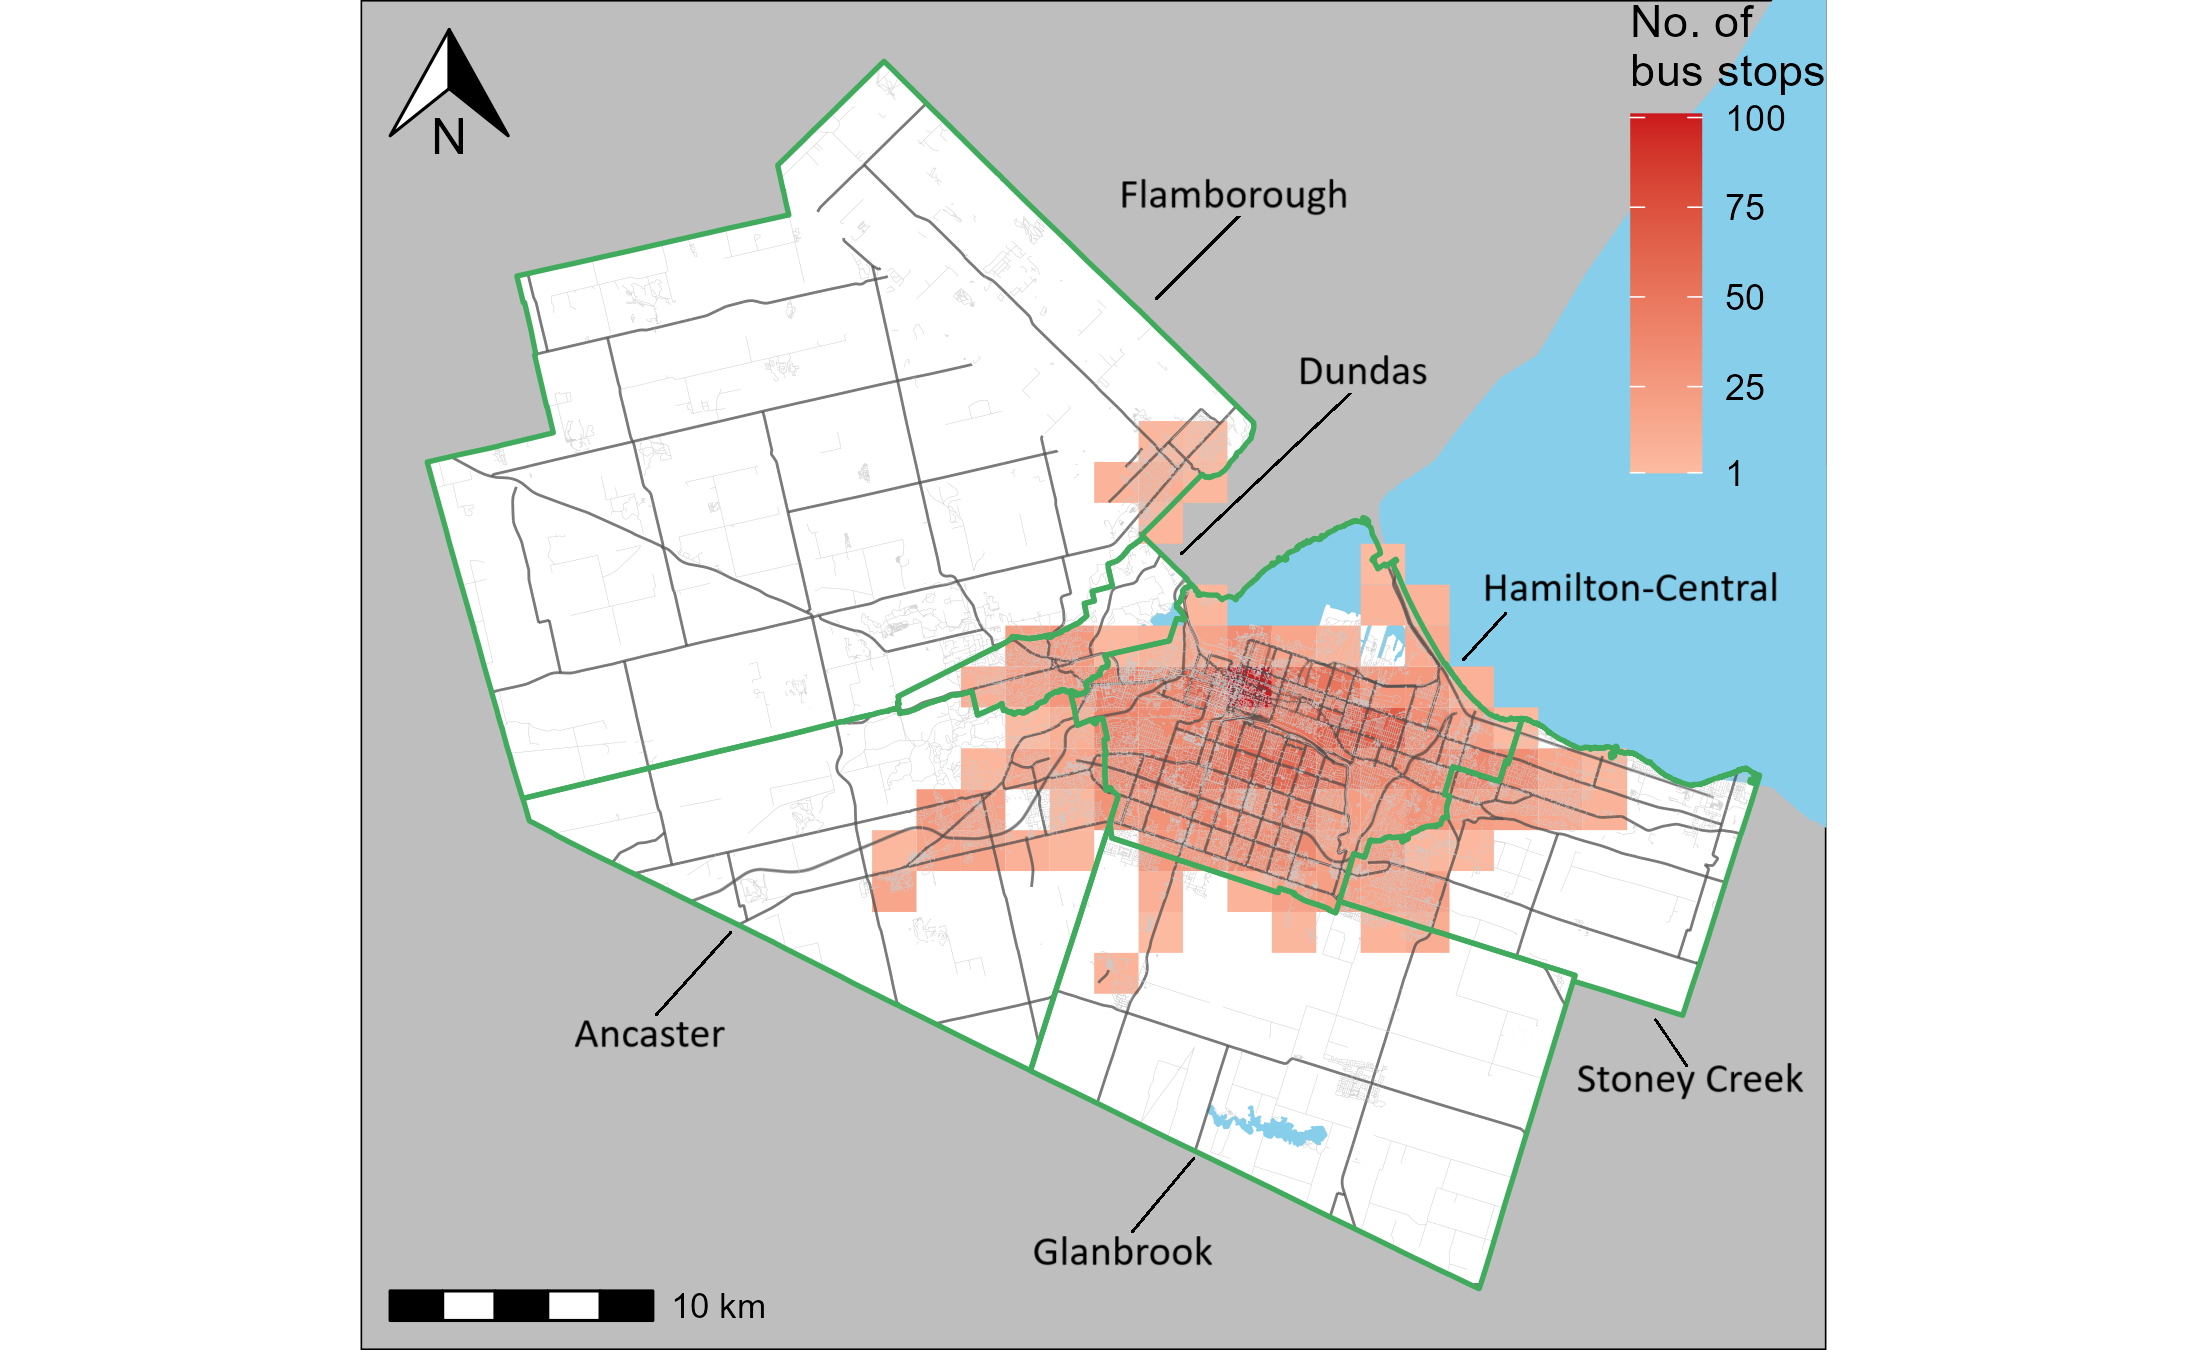
\includegraphics[width=6.25in,height=\textheight]{figures/Fig1-descriptive-boundaries.png}

}

\caption{\label{fig-Fig1}The six former muncipal boundaries in the city
of Hamilton (green), highways and arerial roads (grey), walking and
cycling infrastructure (light grey), and concentration of transit bus
stops (reds). Geographic layer sources: road network
\citep{geofabrikOntarioCanadaOpen2023}, transit stops
\citep{transitfeedsHamiltonStreetRailway2023}, community boundaries
\citep{opendatahamiltonCityBoundary2023} and lake
\citep{greatlakesUSGS2010}.}

\end{figure}%

\subsection{Care destination dataset}\label{care-destination-dataset}

A spatial dataset of care destinations for Hamilton was compiled from
various sources, and destination operation was manually verified using
Google Maps. To showcase the dataset, each type of destination is
grouped into one of five care destination categories. These five
categories were generated by the authors following the travel purpose
categories created in the mobility of care research by
\citet{sanchezdemadariagaMeasuringMobilitiesCare2019}. Notably:
child-centric (destinations for ``childcare'' escorting trips),
elder-centric (common destinations for other escorting trips that are
not childcare-focused), grocery-centric, health-centric, and
errand-centric destinations. The majority of destinations included can
be publicly accessed (e.g., only public schools, grocery stores,
clinics, community centres). However, certain destinations may require a
fee that could be prohibitive for lower-income households (e.g., all
long term care homes, both publicly subsided or private are included in
the dataset). Category sources of data and preparation notes are
detailed in Table~\ref{tbl-Tbl1}. Their spatial distribution and
sub-categories are visualised in Figure~\ref{fig-Fig2}.

\global\setlength{\Oldarrayrulewidth}{\arrayrulewidth}

\global\setlength{\Oldtabcolsep}{\tabcolsep}

\setlength{\tabcolsep}{2pt}

\renewcommand*{\arraystretch}{1.5}



\providecommand{\ascline}[3]{\noalign{\global\arrayrulewidth #1}\arrayrulecolor[HTML]{#2}\cline{#3}}

\begin{longtable}[c]{|p{0.67in}|p{1.69in}|p{4.33in}}

\caption{\label{tbl-Tbl1}Details on the preparation and data sources of
care destinations.}

\tabularnewline

\ascline{1.5pt}{666666}{1-3}

\multicolumn{1}{>{\raggedright}m{\dimexpr 0.67in+0\tabcolsep}}{\textcolor[HTML]{000000}{\fontsize{8}{8}\selectfont{\global\setmainfont{Arial}{Care\ category}}}} & \multicolumn{1}{>{\raggedright}m{\dimexpr 1.69in+0\tabcolsep}}{\textcolor[HTML]{000000}{\fontsize{8}{8}\selectfont{\global\setmainfont{Arial}{Sources}}}} & \multicolumn{1}{>{\raggedright}m{\dimexpr 4.33in+0\tabcolsep}}{\textcolor[HTML]{000000}{\fontsize{8}{8}\selectfont{\global\setmainfont{Arial}{Data\ preparation\ notes}}}} \\

\ascline{1.5pt}{666666}{1-3}\endfirsthead 

\ascline{1.5pt}{666666}{1-3}

\multicolumn{1}{>{\raggedright}m{\dimexpr 0.67in+0\tabcolsep}}{\textcolor[HTML]{000000}{\fontsize{8}{8}\selectfont{\global\setmainfont{Arial}{Care\ category}}}} & \multicolumn{1}{>{\raggedright}m{\dimexpr 1.69in+0\tabcolsep}}{\textcolor[HTML]{000000}{\fontsize{8}{8}\selectfont{\global\setmainfont{Arial}{Sources}}}} & \multicolumn{1}{>{\raggedright}m{\dimexpr 4.33in+0\tabcolsep}}{\textcolor[HTML]{000000}{\fontsize{8}{8}\selectfont{\global\setmainfont{Arial}{Data\ preparation\ notes}}}} \\

\ascline{1.5pt}{666666}{1-3}\endhead



\multicolumn{1}{>{\raggedright}m{\dimexpr 0.67in+0\tabcolsep}}{\textcolor[HTML]{000000}{\fontsize{8}{8}\selectfont{\global\setmainfont{Arial}{Child-centric}}}} & \multicolumn{1}{>{\raggedright}m{\dimexpr 1.69in+0\tabcolsep}}{\textcolor[HTML]{000000}{\fontsize{8}{8}\selectfont{\global\setmainfont{Arial}{(Hamilton}}}\textcolor[HTML]{000000}{\fontsize{8}{8}\selectfont{\global\setmainfont{Arial}{\ }}}\textcolor[HTML]{000000}{\fontsize{8}{8}\selectfont{\global\setmainfont{Arial}{2022a,}}}\textcolor[HTML]{000000}{\fontsize{8}{8}\selectfont{\global\setmainfont{Arial}{\ }}}\textcolor[HTML]{000000}{\fontsize{8}{8}\selectfont{\global\setmainfont{Arial}{2023,}}}\textcolor[HTML]{000000}{\fontsize{8}{8}\selectfont{\global\setmainfont{Arial}{\ }}}\textcolor[HTML]{000000}{\fontsize{8}{8}\selectfont{\global\setmainfont{Arial}{2022c,}}}\textcolor[HTML]{000000}{\fontsize{8}{8}\selectfont{\global\setmainfont{Arial}{\ }}}\textcolor[HTML]{000000}{\fontsize{8}{8}\selectfont{\global\setmainfont{Arial}{2022d;}}}\textcolor[HTML]{000000}{\fontsize{8}{8}\selectfont{\global\setmainfont{Arial}{\ }}}\textcolor[HTML]{000000}{\fontsize{8}{8}\selectfont{\global\setmainfont{Arial}{Ontario}}}\textcolor[HTML]{000000}{\fontsize{8}{8}\selectfont{\global\setmainfont{Arial}{\ }}}\textcolor[HTML]{000000}{\fontsize{8}{8}\selectfont{\global\setmainfont{Arial}{2023b)}}}} & \multicolumn{1}{>{\raggedright}m{\dimexpr 4.33in+0\tabcolsep}}{\textcolor[HTML]{000000}{\fontsize{8}{8}\selectfont{\global\setmainfont{Arial}{Public}}}\textcolor[HTML]{000000}{\fontsize{8}{8}\selectfont{\global\setmainfont{Arial}{\ }}}\textcolor[HTML]{000000}{\fontsize{8}{8}\selectfont{\global\setmainfont{Arial}{schools,}}}\textcolor[HTML]{000000}{\fontsize{8}{8}\selectfont{\global\setmainfont{Arial}{\ }}}\textcolor[HTML]{000000}{\fontsize{8}{8}\selectfont{\global\setmainfont{Arial}{public}}}\textcolor[HTML]{000000}{\fontsize{8}{8}\selectfont{\global\setmainfont{Arial}{\ }}}\textcolor[HTML]{000000}{\fontsize{8}{8}\selectfont{\global\setmainfont{Arial}{and}}}\textcolor[HTML]{000000}{\fontsize{8}{8}\selectfont{\global\setmainfont{Arial}{\ }}}\textcolor[HTML]{000000}{\fontsize{8}{8}\selectfont{\global\setmainfont{Arial}{private}}}\textcolor[HTML]{000000}{\fontsize{8}{8}\selectfont{\global\setmainfont{Arial}{\ }}}\textcolor[HTML]{000000}{\fontsize{8}{8}\selectfont{\global\setmainfont{Arial}{(licensed)}}}\textcolor[HTML]{000000}{\fontsize{8}{8}\selectfont{\global\setmainfont{Arial}{\ }}}\textcolor[HTML]{000000}{\fontsize{8}{8}\selectfont{\global\setmainfont{Arial}{daycares,}}}\textcolor[HTML]{000000}{\fontsize{8}{8}\selectfont{\global\setmainfont{Arial}{\ }}}\textcolor[HTML]{000000}{\fontsize{8}{8}\selectfont{\global\setmainfont{Arial}{and}}}\textcolor[HTML]{000000}{\fontsize{8}{8}\selectfont{\global\setmainfont{Arial}{\ }}}\textcolor[HTML]{000000}{\fontsize{8}{8}\selectfont{\global\setmainfont{Arial}{public}}}\textcolor[HTML]{000000}{\fontsize{8}{8}\selectfont{\global\setmainfont{Arial}{\ }}}\textcolor[HTML]{000000}{\fontsize{8}{8}\selectfont{\global\setmainfont{Arial}{community}}}\textcolor[HTML]{000000}{\fontsize{8}{8}\selectfont{\global\setmainfont{Arial}{\ }}}\textcolor[HTML]{000000}{\fontsize{8}{8}\selectfont{\global\setmainfont{Arial}{centres,}}}\textcolor[HTML]{000000}{\fontsize{8}{8}\selectfont{\global\setmainfont{Arial}{\ }}}\textcolor[HTML]{000000}{\fontsize{8}{8}\selectfont{\global\setmainfont{Arial}{public}}}\textcolor[HTML]{000000}{\fontsize{8}{8}\selectfont{\global\setmainfont{Arial}{\ }}}\textcolor[HTML]{000000}{\fontsize{8}{8}\selectfont{\global\setmainfont{Arial}{recreation}}}\textcolor[HTML]{000000}{\fontsize{8}{8}\selectfont{\global\setmainfont{Arial}{\ }}}\textcolor[HTML]{000000}{\fontsize{8}{8}\selectfont{\global\setmainfont{Arial}{centres,}}}\textcolor[HTML]{000000}{\fontsize{8}{8}\selectfont{\global\setmainfont{Arial}{\ }}}\textcolor[HTML]{000000}{\fontsize{8}{8}\selectfont{\global\setmainfont{Arial}{and}}}\textcolor[HTML]{000000}{\fontsize{8}{8}\selectfont{\global\setmainfont{Arial}{\ }}}\textcolor[HTML]{000000}{\fontsize{8}{8}\selectfont{\global\setmainfont{Arial}{public}}}\textcolor[HTML]{000000}{\fontsize{8}{8}\selectfont{\global\setmainfont{Arial}{\ }}}\textcolor[HTML]{000000}{\fontsize{8}{8}\selectfont{\global\setmainfont{Arial}{parks:}}}\textcolor[HTML]{000000}{\fontsize{8}{8}\selectfont{\global\setmainfont{Arial}{\ }}}\textcolor[HTML]{000000}{\fontsize{8}{8}\selectfont{\global\setmainfont{Arial}{1,190}}}\textcolor[HTML]{000000}{\fontsize{8}{8}\selectfont{\global\setmainfont{Arial}{\ }}}\textcolor[HTML]{000000}{\fontsize{8}{8}\selectfont{\global\setmainfont{Arial}{locations}}}\textcolor[HTML]{000000}{\fontsize{8}{8}\selectfont{\global\setmainfont{Arial}{\ }}}\textcolor[HTML]{000000}{\fontsize{8}{8}\selectfont{\global\setmainfont{Arial}{are}}}\textcolor[HTML]{000000}{\fontsize{8}{8}\selectfont{\global\setmainfont{Arial}{\ }}}\textcolor[HTML]{000000}{\fontsize{8}{8}\selectfont{\global\setmainfont{Arial}{included.}}}\textcolor[HTML]{000000}{\fontsize{8}{8}\selectfont{\global\setmainfont{Arial}{\ }}}\textcolor[HTML]{000000}{\fontsize{8}{8}\selectfont{\global\setmainfont{Arial}{After}}}\textcolor[HTML]{000000}{\fontsize{8}{8}\selectfont{\global\setmainfont{Arial}{\ }}}\textcolor[HTML]{000000}{\fontsize{8}{8}\selectfont{\global\setmainfont{Arial}{manual}}}\textcolor[HTML]{000000}{\fontsize{8}{8}\selectfont{\global\setmainfont{Arial}{\ }}}\textcolor[HTML]{000000}{\fontsize{8}{8}\selectfont{\global\setmainfont{Arial}{review,}}}\textcolor[HTML]{000000}{\fontsize{8}{8}\selectfont{\global\setmainfont{Arial}{\ }}}\textcolor[HTML]{000000}{\fontsize{8}{8}\selectfont{\global\setmainfont{Arial}{all}}}\textcolor[HTML]{000000}{\fontsize{8}{8}\selectfont{\global\setmainfont{Arial}{\ }}}\textcolor[HTML]{000000}{\fontsize{8}{8}\selectfont{\global\setmainfont{Arial}{locations}}}\textcolor[HTML]{000000}{\fontsize{8}{8}\selectfont{\global\setmainfont{Arial}{\ }}}\textcolor[HTML]{000000}{\fontsize{8}{8}\selectfont{\global\setmainfont{Arial}{that}}}\textcolor[HTML]{000000}{\fontsize{8}{8}\selectfont{\global\setmainfont{Arial}{\ }}}\textcolor[HTML]{000000}{\fontsize{8}{8}\selectfont{\global\setmainfont{Arial}{typically}}}\textcolor[HTML]{000000}{\fontsize{8}{8}\selectfont{\global\setmainfont{Arial}{\ }}}\textcolor[HTML]{000000}{\fontsize{8}{8}\selectfont{\global\setmainfont{Arial}{do}}}\textcolor[HTML]{000000}{\fontsize{8}{8}\selectfont{\global\setmainfont{Arial}{\ }}}\textcolor[HTML]{000000}{\fontsize{8}{8}\selectfont{\global\setmainfont{Arial}{not}}}\textcolor[HTML]{000000}{\fontsize{8}{8}\selectfont{\global\setmainfont{Arial}{\ }}}\textcolor[HTML]{000000}{\fontsize{8}{8}\selectfont{\global\setmainfont{Arial}{serve}}}\textcolor[HTML]{000000}{\fontsize{8}{8}\selectfont{\global\setmainfont{Arial}{\ }}}\textcolor[HTML]{000000}{\fontsize{8}{8}\selectfont{\global\setmainfont{Arial}{children}}}\textcolor[HTML]{000000}{\fontsize{8}{8}\selectfont{\global\setmainfont{Arial}{\ }}}\textcolor[HTML]{000000}{\fontsize{8}{8}\selectfont{\global\setmainfont{Arial}{were}}}\textcolor[HTML]{000000}{\fontsize{8}{8}\selectfont{\global\setmainfont{Arial}{\ }}}\textcolor[HTML]{000000}{\fontsize{8}{8}\selectfont{\global\setmainfont{Arial}{removed}}}\textcolor[HTML]{000000}{\fontsize{8}{8}\selectfont{\global\setmainfont{Arial}{\ }}}\textcolor[HTML]{000000}{\fontsize{8}{8}\selectfont{\global\setmainfont{Arial}{including:}}}\textcolor[HTML]{000000}{\fontsize{8}{8}\selectfont{\global\setmainfont{Arial}{\ }}}\textcolor[HTML]{000000}{\fontsize{8}{8}\selectfont{\global\setmainfont{Arial}{Post-Secondary,}}}\textcolor[HTML]{000000}{\fontsize{8}{8}\selectfont{\global\setmainfont{Arial}{\ }}}\textcolor[HTML]{000000}{\fontsize{8}{8}\selectfont{\global\setmainfont{Arial}{Adult-Learning}}}\textcolor[HTML]{000000}{\fontsize{8}{8}\selectfont{\global\setmainfont{Arial}{\ }}}\textcolor[HTML]{000000}{\fontsize{8}{8}\selectfont{\global\setmainfont{Arial}{Centres,}}}\textcolor[HTML]{000000}{\fontsize{8}{8}\selectfont{\global\setmainfont{Arial}{\ }}}\textcolor[HTML]{000000}{\fontsize{8}{8}\selectfont{\global\setmainfont{Arial}{Group}}}\textcolor[HTML]{000000}{\fontsize{8}{8}\selectfont{\global\setmainfont{Arial}{\ }}}\textcolor[HTML]{000000}{\fontsize{8}{8}\selectfont{\global\setmainfont{Arial}{Homes,}}}\textcolor[HTML]{000000}{\fontsize{8}{8}\selectfont{\global\setmainfont{Arial}{\ }}}\textcolor[HTML]{000000}{\fontsize{8}{8}\selectfont{\global\setmainfont{Arial}{and}}}\textcolor[HTML]{000000}{\fontsize{8}{8}\selectfont{\global\setmainfont{Arial}{\ }}}\textcolor[HTML]{000000}{\fontsize{8}{8}\selectfont{\global\setmainfont{Arial}{Foster}}}\textcolor[HTML]{000000}{\fontsize{8}{8}\selectfont{\global\setmainfont{Arial}{\ }}}\textcolor[HTML]{000000}{\fontsize{8}{8}\selectfont{\global\setmainfont{Arial}{Care}}}\textcolor[HTML]{000000}{\fontsize{8}{8}\selectfont{\global\setmainfont{Arial}{\ }}}\textcolor[HTML]{000000}{\fontsize{8}{8}\selectfont{\global\setmainfont{Arial}{Centres.}}}\textcolor[HTML]{000000}{\fontsize{8}{8}\selectfont{\global\setmainfont{Arial}{\ }}}\textcolor[HTML]{000000}{\fontsize{8}{8}\selectfont{\global\setmainfont{Arial}{Further,}}}\textcolor[HTML]{000000}{\fontsize{8}{8}\selectfont{\global\setmainfont{Arial}{\ }}}\textcolor[HTML]{000000}{\fontsize{8}{8}\selectfont{\global\setmainfont{Arial}{through}}}\textcolor[HTML]{000000}{\fontsize{8}{8}\selectfont{\global\setmainfont{Arial}{\ }}}\textcolor[HTML]{000000}{\fontsize{8}{8}\selectfont{\global\setmainfont{Arial}{examination}}}\textcolor[HTML]{000000}{\fontsize{8}{8}\selectfont{\global\setmainfont{Arial}{\ }}}\textcolor[HTML]{000000}{\fontsize{8}{8}\selectfont{\global\setmainfont{Arial}{some}}}\textcolor[HTML]{000000}{\fontsize{8}{8}\selectfont{\global\setmainfont{Arial}{\ }}}\textcolor[HTML]{000000}{\fontsize{8}{8}\selectfont{\global\setmainfont{Arial}{Section}}}\textcolor[HTML]{000000}{\fontsize{8}{8}\selectfont{\global\setmainfont{Arial}{\ }}}\textcolor[HTML]{000000}{\fontsize{8}{8}\selectfont{\global\setmainfont{Arial}{23}}}\textcolor[HTML]{000000}{\fontsize{8}{8}\selectfont{\global\setmainfont{Arial}{\ }}}\textcolor[HTML]{000000}{\fontsize{8}{8}\selectfont{\global\setmainfont{Arial}{institutions}}}\textcolor[HTML]{000000}{\fontsize{8}{8}\selectfont{\global\setmainfont{Arial}{\ }}}\textcolor[HTML]{000000}{\fontsize{8}{8}\selectfont{\global\setmainfont{Arial}{defined}}}\textcolor[HTML]{000000}{\fontsize{8}{8}\selectfont{\global\setmainfont{Arial}{\ }}}\textcolor[HTML]{000000}{\fontsize{8}{8}\selectfont{\global\setmainfont{Arial}{as}}}\textcolor[HTML]{000000}{\fontsize{8}{8}\selectfont{\global\setmainfont{Arial}{\ }}}\textcolor[HTML]{000000}{\fontsize{8}{8}\selectfont{\global\setmainfont{Arial}{\textit{“}}}}\textcolor[HTML]{000000}{\fontsize{8}{8}\selectfont{\global\setmainfont{Arial}{\textit{centres}}}}\textcolor[HTML]{000000}{\fontsize{8}{8}\selectfont{\global\setmainfont{Arial}{\textit{\ }}}}\textcolor[HTML]{000000}{\fontsize{8}{8}\selectfont{\global\setmainfont{Arial}{\textit{for}}}}\textcolor[HTML]{000000}{\fontsize{8}{8}\selectfont{\global\setmainfont{Arial}{\textit{\ }}}}\textcolor[HTML]{000000}{\fontsize{8}{8}\selectfont{\global\setmainfont{Arial}{\textit{children}}}}\textcolor[HTML]{000000}{\fontsize{8}{8}\selectfont{\global\setmainfont{Arial}{\textit{\ }}}}\textcolor[HTML]{000000}{\fontsize{8}{8}\selectfont{\global\setmainfont{Arial}{\textit{who}}}}\textcolor[HTML]{000000}{\fontsize{8}{8}\selectfont{\global\setmainfont{Arial}{\textit{\ }}}}\textcolor[HTML]{000000}{\fontsize{8}{8}\selectfont{\global\setmainfont{Arial}{\textit{cannot}}}}\textcolor[HTML]{000000}{\fontsize{8}{8}\selectfont{\global\setmainfont{Arial}{\textit{\ }}}}\textcolor[HTML]{000000}{\fontsize{8}{8}\selectfont{\global\setmainfont{Arial}{\textit{attend}}}}\textcolor[HTML]{000000}{\fontsize{8}{8}\selectfont{\global\setmainfont{Arial}{\textit{\ }}}}\textcolor[HTML]{000000}{\fontsize{8}{8}\selectfont{\global\setmainfont{Arial}{\textit{school}}}}\textcolor[HTML]{000000}{\fontsize{8}{8}\selectfont{\global\setmainfont{Arial}{\textit{\ }}}}\textcolor[HTML]{000000}{\fontsize{8}{8}\selectfont{\global\setmainfont{Arial}{\textit{to}}}}\textcolor[HTML]{000000}{\fontsize{8}{8}\selectfont{\global\setmainfont{Arial}{\textit{\ }}}}\textcolor[HTML]{000000}{\fontsize{8}{8}\selectfont{\global\setmainfont{Arial}{\textit{meet}}}}\textcolor[HTML]{000000}{\fontsize{8}{8}\selectfont{\global\setmainfont{Arial}{\textit{\ }}}}\textcolor[HTML]{000000}{\fontsize{8}{8}\selectfont{\global\setmainfont{Arial}{\textit{the}}}}\textcolor[HTML]{000000}{\fontsize{8}{8}\selectfont{\global\setmainfont{Arial}{\textit{\ }}}}\textcolor[HTML]{000000}{\fontsize{8}{8}\selectfont{\global\setmainfont{Arial}{\textit{needs}}}}\textcolor[HTML]{000000}{\fontsize{8}{8}\selectfont{\global\setmainfont{Arial}{\textit{\ }}}}\textcolor[HTML]{000000}{\fontsize{8}{8}\selectfont{\global\setmainfont{Arial}{\textit{of}}}}\textcolor[HTML]{000000}{\fontsize{8}{8}\selectfont{\global\setmainfont{Arial}{\textit{\ }}}}\textcolor[HTML]{000000}{\fontsize{8}{8}\selectfont{\global\setmainfont{Arial}{\textit{care}}}}\textcolor[HTML]{000000}{\fontsize{8}{8}\selectfont{\global\setmainfont{Arial}{\textit{\ }}}}\textcolor[HTML]{000000}{\fontsize{8}{8}\selectfont{\global\setmainfont{Arial}{\textit{or}}}}\textcolor[HTML]{000000}{\fontsize{8}{8}\selectfont{\global\setmainfont{Arial}{\textit{\ }}}}\textcolor[HTML]{000000}{\fontsize{8}{8}\selectfont{\global\setmainfont{Arial}{\textit{treatment,}}}}\textcolor[HTML]{000000}{\fontsize{8}{8}\selectfont{\global\setmainfont{Arial}{\textit{\ }}}}\textcolor[HTML]{000000}{\fontsize{8}{8}\selectfont{\global\setmainfont{Arial}{\textit{and}}}}\textcolor[HTML]{000000}{\fontsize{8}{8}\selectfont{\global\setmainfont{Arial}{\textit{\ }}}}\textcolor[HTML]{000000}{\fontsize{8}{8}\selectfont{\global\setmainfont{Arial}{\textit{rehabilitation}}}}\textcolor[HTML]{000000}{\fontsize{8}{8}\selectfont{\global\setmainfont{Arial}{\textit{”}}}}\textcolor[HTML]{000000}{\fontsize{8}{8}\selectfont{\global\setmainfont{Arial}{\ }}}\textcolor[HTML]{000000}{\fontsize{8}{8}\selectfont{\global\setmainfont{Arial}{(Ontario}}}\textcolor[HTML]{000000}{\fontsize{8}{8}\selectfont{\global\setmainfont{Arial}{\ }}}\textcolor[HTML]{000000}{\fontsize{8}{8}\selectfont{\global\setmainfont{Arial}{2023a)}}}\textcolor[HTML]{000000}{\fontsize{8}{8}\selectfont{\global\setmainfont{Arial}{,}}}\textcolor[HTML]{000000}{\fontsize{8}{8}\selectfont{\global\setmainfont{Arial}{\ }}}\textcolor[HTML]{000000}{\fontsize{8}{8}\selectfont{\global\setmainfont{Arial}{were}}}\textcolor[HTML]{000000}{\fontsize{8}{8}\selectfont{\global\setmainfont{Arial}{\ }}}\textcolor[HTML]{000000}{\fontsize{8}{8}\selectfont{\global\setmainfont{Arial}{kept}}}\textcolor[HTML]{000000}{\fontsize{8}{8}\selectfont{\global\setmainfont{Arial}{\ }}}\textcolor[HTML]{000000}{\fontsize{8}{8}\selectfont{\global\setmainfont{Arial}{due}}}\textcolor[HTML]{000000}{\fontsize{8}{8}\selectfont{\global\setmainfont{Arial}{\ }}}\textcolor[HTML]{000000}{\fontsize{8}{8}\selectfont{\global\setmainfont{Arial}{to}}}\textcolor[HTML]{000000}{\fontsize{8}{8}\selectfont{\global\setmainfont{Arial}{\ }}}\textcolor[HTML]{000000}{\fontsize{8}{8}\selectfont{\global\setmainfont{Arial}{their}}}\textcolor[HTML]{000000}{\fontsize{8}{8}\selectfont{\global\setmainfont{Arial}{\ }}}\textcolor[HTML]{000000}{\fontsize{8}{8}\selectfont{\global\setmainfont{Arial}{innate}}}\textcolor[HTML]{000000}{\fontsize{8}{8}\selectfont{\global\setmainfont{Arial}{\ }}}\textcolor[HTML]{000000}{\fontsize{8}{8}\selectfont{\global\setmainfont{Arial}{connection}}}\textcolor[HTML]{000000}{\fontsize{8}{8}\selectfont{\global\setmainfont{Arial}{\ }}}\textcolor[HTML]{000000}{\fontsize{8}{8}\selectfont{\global\setmainfont{Arial}{to}}}\textcolor[HTML]{000000}{\fontsize{8}{8}\selectfont{\global\setmainfont{Arial}{\ }}}\textcolor[HTML]{000000}{\fontsize{8}{8}\selectfont{\global\setmainfont{Arial}{care.}}}} \\





\multicolumn{1}{>{\raggedright}m{\dimexpr 0.67in+0\tabcolsep}}{\textcolor[HTML]{000000}{\fontsize{8}{8}\selectfont{\global\setmainfont{Arial}{Elder-centric}}}} & \multicolumn{1}{>{\raggedright}m{\dimexpr 1.69in+0\tabcolsep}}{\textcolor[HTML]{000000}{\fontsize{8}{8}\selectfont{\global\setmainfont{Arial}{(Hamilton}}}\textcolor[HTML]{000000}{\fontsize{8}{8}\selectfont{\global\setmainfont{Arial}{\ }}}\textcolor[HTML]{000000}{\fontsize{8}{8}\selectfont{\global\setmainfont{Arial}{2022d;}}}\textcolor[HTML]{000000}{\fontsize{8}{8}\selectfont{\global\setmainfont{Arial}{\ }}}\textcolor[HTML]{000000}{\fontsize{8}{8}\selectfont{\global\setmainfont{Arial}{Ontario GeoHub}}}\textcolor[HTML]{000000}{\fontsize{8}{8}\selectfont{\global\setmainfont{Arial}{\ }}}\textcolor[HTML]{000000}{\fontsize{8}{8}\selectfont{\global\setmainfont{Arial}{2023)}}}} & \multicolumn{1}{>{\raggedright}m{\dimexpr 4.33in+0\tabcolsep}}{\textcolor[HTML]{000000}{\fontsize{8}{8}\selectfont{\global\setmainfont{Arial}{Public}}}\textcolor[HTML]{000000}{\fontsize{8}{8}\selectfont{\global\setmainfont{Arial}{\ }}}\textcolor[HTML]{000000}{\fontsize{8}{8}\selectfont{\global\setmainfont{Arial}{and}}}\textcolor[HTML]{000000}{\fontsize{8}{8}\selectfont{\global\setmainfont{Arial}{\ }}}\textcolor[HTML]{000000}{\fontsize{8}{8}\selectfont{\global\setmainfont{Arial}{private}}}\textcolor[HTML]{000000}{\fontsize{8}{8}\selectfont{\global\setmainfont{Arial}{\ }}}\textcolor[HTML]{000000}{\fontsize{8}{8}\selectfont{\global\setmainfont{Arial}{senior}}}\textcolor[HTML]{000000}{\fontsize{8}{8}\selectfont{\global\setmainfont{Arial}{\ }}}\textcolor[HTML]{000000}{\fontsize{8}{8}\selectfont{\global\setmainfont{Arial}{centres,}}}\textcolor[HTML]{000000}{\fontsize{8}{8}\selectfont{\global\setmainfont{Arial}{\ }}}\textcolor[HTML]{000000}{\fontsize{8}{8}\selectfont{\global\setmainfont{Arial}{long-term}}}\textcolor[HTML]{000000}{\fontsize{8}{8}\selectfont{\global\setmainfont{Arial}{\ }}}\textcolor[HTML]{000000}{\fontsize{8}{8}\selectfont{\global\setmainfont{Arial}{care}}}\textcolor[HTML]{000000}{\fontsize{8}{8}\selectfont{\global\setmainfont{Arial}{\ }}}\textcolor[HTML]{000000}{\fontsize{8}{8}\selectfont{\global\setmainfont{Arial}{homes,}}}\textcolor[HTML]{000000}{\fontsize{8}{8}\selectfont{\global\setmainfont{Arial}{\ }}}\textcolor[HTML]{000000}{\fontsize{8}{8}\selectfont{\global\setmainfont{Arial}{and}}}\textcolor[HTML]{000000}{\fontsize{8}{8}\selectfont{\global\setmainfont{Arial}{\ }}}\textcolor[HTML]{000000}{\fontsize{8}{8}\selectfont{\global\setmainfont{Arial}{retirement}}}\textcolor[HTML]{000000}{\fontsize{8}{8}\selectfont{\global\setmainfont{Arial}{\ }}}\textcolor[HTML]{000000}{\fontsize{8}{8}\selectfont{\global\setmainfont{Arial}{homes:}}}\textcolor[HTML]{000000}{\fontsize{8}{8}\selectfont{\global\setmainfont{Arial}{\ }}}\textcolor[HTML]{000000}{\fontsize{8}{8}\selectfont{\global\setmainfont{Arial}{75}}}\textcolor[HTML]{000000}{\fontsize{8}{8}\selectfont{\global\setmainfont{Arial}{\ }}}\textcolor[HTML]{000000}{\fontsize{8}{8}\selectfont{\global\setmainfont{Arial}{destinations}}}\textcolor[HTML]{000000}{\fontsize{8}{8}\selectfont{\global\setmainfont{Arial}{\ }}}\textcolor[HTML]{000000}{\fontsize{8}{8}\selectfont{\global\setmainfont{Arial}{are}}}\textcolor[HTML]{000000}{\fontsize{8}{8}\selectfont{\global\setmainfont{Arial}{\ }}}\textcolor[HTML]{000000}{\fontsize{8}{8}\selectfont{\global\setmainfont{Arial}{identified.}}}} \\





\multicolumn{1}{>{\raggedright}m{\dimexpr 0.67in+0\tabcolsep}}{\textcolor[HTML]{000000}{\fontsize{8}{8}\selectfont{\global\setmainfont{Arial}{Grocery-centric}}}} & \multicolumn{1}{>{\raggedright}m{\dimexpr 1.69in+0\tabcolsep}}{\textcolor[HTML]{000000}{\fontsize{8}{8}\selectfont{\global\setmainfont{Arial}{(Axle Data}}}\textcolor[HTML]{000000}{\fontsize{8}{8}\selectfont{\global\setmainfont{Arial}{\ }}}\textcolor[HTML]{000000}{\fontsize{8}{8}\selectfont{\global\setmainfont{Arial}{2023)}}}} & \multicolumn{1}{>{\raggedright}m{\dimexpr 4.33in+0\tabcolsep}}{\textcolor[HTML]{000000}{\fontsize{8}{8}\selectfont{\global\setmainfont{Arial}{Grocery}}}\textcolor[HTML]{000000}{\fontsize{8}{8}\selectfont{\global\setmainfont{Arial}{\ }}}\textcolor[HTML]{000000}{\fontsize{8}{8}\selectfont{\global\setmainfont{Arial}{stores,}}}\textcolor[HTML]{000000}{\fontsize{8}{8}\selectfont{\global\setmainfont{Arial}{\ }}}\textcolor[HTML]{000000}{\fontsize{8}{8}\selectfont{\global\setmainfont{Arial}{namely}}}\textcolor[HTML]{000000}{\fontsize{8}{8}\selectfont{\global\setmainfont{Arial}{\ }}}\textcolor[HTML]{000000}{\fontsize{8}{8}\selectfont{\global\setmainfont{Arial}{a}}}\textcolor[HTML]{000000}{\fontsize{8}{8}\selectfont{\global\setmainfont{Arial}{\ }}}\textcolor[HTML]{000000}{\fontsize{8}{8}\selectfont{\global\setmainfont{Arial}{place}}}\textcolor[HTML]{000000}{\fontsize{8}{8}\selectfont{\global\setmainfont{Arial}{\ }}}\textcolor[HTML]{000000}{\fontsize{8}{8}\selectfont{\global\setmainfont{Arial}{a}}}\textcolor[HTML]{000000}{\fontsize{8}{8}\selectfont{\global\setmainfont{Arial}{\ }}}\textcolor[HTML]{000000}{\fontsize{8}{8}\selectfont{\global\setmainfont{Arial}{household}}}\textcolor[HTML]{000000}{\fontsize{8}{8}\selectfont{\global\setmainfont{Arial}{\ }}}\textcolor[HTML]{000000}{\fontsize{8}{8}\selectfont{\global\setmainfont{Arial}{could}}}\textcolor[HTML]{000000}{\fontsize{8}{8}\selectfont{\global\setmainfont{Arial}{\ }}}\textcolor[HTML]{000000}{\fontsize{8}{8}\selectfont{\global\setmainfont{Arial}{buy}}}\textcolor[HTML]{000000}{\fontsize{8}{8}\selectfont{\global\setmainfont{Arial}{\ }}}\textcolor[HTML]{000000}{\fontsize{8}{8}\selectfont{\global\setmainfont{Arial}{groceries}}}\textcolor[HTML]{000000}{\fontsize{8}{8}\selectfont{\global\setmainfont{Arial}{\ }}}\textcolor[HTML]{000000}{\fontsize{8}{8}\selectfont{\global\setmainfont{Arial}{ranging}}}\textcolor[HTML]{000000}{\fontsize{8}{8}\selectfont{\global\setmainfont{Arial}{\ }}}\textcolor[HTML]{000000}{\fontsize{8}{8}\selectfont{\global\setmainfont{Arial}{from}}}\textcolor[HTML]{000000}{\fontsize{8}{8}\selectfont{\global\setmainfont{Arial}{\ }}}\textcolor[HTML]{000000}{\fontsize{8}{8}\selectfont{\global\setmainfont{Arial}{convenience}}}\textcolor[HTML]{000000}{\fontsize{8}{8}\selectfont{\global\setmainfont{Arial}{\ }}}\textcolor[HTML]{000000}{\fontsize{8}{8}\selectfont{\global\setmainfont{Arial}{stores}}}\textcolor[HTML]{000000}{\fontsize{8}{8}\selectfont{\global\setmainfont{Arial}{\ }}}\textcolor[HTML]{000000}{\fontsize{8}{8}\selectfont{\global\setmainfont{Arial}{to}}}\textcolor[HTML]{000000}{\fontsize{8}{8}\selectfont{\global\setmainfont{Arial}{\ }}}\textcolor[HTML]{000000}{\fontsize{8}{8}\selectfont{\global\setmainfont{Arial}{large}}}\textcolor[HTML]{000000}{\fontsize{8}{8}\selectfont{\global\setmainfont{Arial}{\ }}}\textcolor[HTML]{000000}{\fontsize{8}{8}\selectfont{\global\setmainfont{Arial}{retail}}}\textcolor[HTML]{000000}{\fontsize{8}{8}\selectfont{\global\setmainfont{Arial}{\ }}}\textcolor[HTML]{000000}{\fontsize{8}{8}\selectfont{\global\setmainfont{Arial}{stores:}}}\textcolor[HTML]{000000}{\fontsize{8}{8}\selectfont{\global\setmainfont{Arial}{\ }}}\textcolor[HTML]{000000}{\fontsize{8}{8}\selectfont{\global\setmainfont{Arial}{381}}}\textcolor[HTML]{000000}{\fontsize{8}{8}\selectfont{\global\setmainfont{Arial}{\ }}}\textcolor[HTML]{000000}{\fontsize{8}{8}\selectfont{\global\setmainfont{Arial}{destinations}}}\textcolor[HTML]{000000}{\fontsize{8}{8}\selectfont{\global\setmainfont{Arial}{\ }}}\textcolor[HTML]{000000}{\fontsize{8}{8}\selectfont{\global\setmainfont{Arial}{are}}}\textcolor[HTML]{000000}{\fontsize{8}{8}\selectfont{\global\setmainfont{Arial}{\ }}}\textcolor[HTML]{000000}{\fontsize{8}{8}\selectfont{\global\setmainfont{Arial}{identified.}}}\textcolor[HTML]{000000}{\fontsize{8}{8}\selectfont{\global\setmainfont{Arial}{\ }}}\textcolor[HTML]{000000}{\fontsize{8}{8}\selectfont{\global\setmainfont{Arial}{Data}}}\textcolor[HTML]{000000}{\fontsize{8}{8}\selectfont{\global\setmainfont{Arial}{\ }}}\textcolor[HTML]{000000}{\fontsize{8}{8}\selectfont{\global\setmainfont{Arial}{is}}}\textcolor[HTML]{000000}{\fontsize{8}{8}\selectfont{\global\setmainfont{Arial}{\ }}}\textcolor[HTML]{000000}{\fontsize{8}{8}\selectfont{\global\setmainfont{Arial}{filtered}}}\textcolor[HTML]{000000}{\fontsize{8}{8}\selectfont{\global\setmainfont{Arial}{\ }}}\textcolor[HTML]{000000}{\fontsize{8}{8}\selectfont{\global\setmainfont{Arial}{by}}}\textcolor[HTML]{000000}{\fontsize{8}{8}\selectfont{\global\setmainfont{Arial}{\ }}}\textcolor[HTML]{000000}{\fontsize{8}{8}\selectfont{\global\setmainfont{Arial}{Company}}}\textcolor[HTML]{000000}{\fontsize{8}{8}\selectfont{\global\setmainfont{Arial}{\ }}}\textcolor[HTML]{000000}{\fontsize{8}{8}\selectfont{\global\setmainfont{Arial}{Name,}}}\textcolor[HTML]{000000}{\fontsize{8}{8}\selectfont{\global\setmainfont{Arial}{\ }}}\textcolor[HTML]{000000}{\fontsize{8}{8}\selectfont{\global\setmainfont{Arial}{Suite}}}\textcolor[HTML]{000000}{\fontsize{8}{8}\selectfont{\global\setmainfont{Arial}{\ }}}\textcolor[HTML]{000000}{\fontsize{8}{8}\selectfont{\global\setmainfont{Arial}{Number,}}}\textcolor[HTML]{000000}{\fontsize{8}{8}\selectfont{\global\setmainfont{Arial}{\ }}}\textcolor[HTML]{000000}{\fontsize{8}{8}\selectfont{\global\setmainfont{Arial}{Address,}}}\textcolor[HTML]{000000}{\fontsize{8}{8}\selectfont{\global\setmainfont{Arial}{\ }}}\textcolor[HTML]{000000}{\fontsize{8}{8}\selectfont{\global\setmainfont{Arial}{City,}}}\textcolor[HTML]{000000}{\fontsize{8}{8}\selectfont{\global\setmainfont{Arial}{\ }}}\textcolor[HTML]{000000}{\fontsize{8}{8}\selectfont{\global\setmainfont{Arial}{Province,}}}\textcolor[HTML]{000000}{\fontsize{8}{8}\selectfont{\global\setmainfont{Arial}{\ }}}\textcolor[HTML]{000000}{\fontsize{8}{8}\selectfont{\global\setmainfont{Arial}{Phone}}}\textcolor[HTML]{000000}{\fontsize{8}{8}\selectfont{\global\setmainfont{Arial}{\ }}}\textcolor[HTML]{000000}{\fontsize{8}{8}\selectfont{\global\setmainfont{Arial}{Number}}}\textcolor[HTML]{000000}{\fontsize{8}{8}\selectfont{\global\setmainfont{Arial}{\ }}}\textcolor[HTML]{000000}{\fontsize{8}{8}\selectfont{\global\setmainfont{Arial}{and}}}\textcolor[HTML]{000000}{\fontsize{8}{8}\selectfont{\global\setmainfont{Arial}{\ }}}\textcolor[HTML]{000000}{\fontsize{8}{8}\selectfont{\global\setmainfont{Arial}{Postal}}}\textcolor[HTML]{000000}{\fontsize{8}{8}\selectfont{\global\setmainfont{Arial}{\ }}}\textcolor[HTML]{000000}{\fontsize{8}{8}\selectfont{\global\setmainfont{Arial}{Code.}}}\textcolor[HTML]{000000}{\fontsize{8}{8}\selectfont{\global\setmainfont{Arial}{\ }}}\textcolor[HTML]{000000}{\fontsize{8}{8}\selectfont{\global\setmainfont{Arial}{The}}}\textcolor[HTML]{000000}{\fontsize{8}{8}\selectfont{\global\setmainfont{Arial}{\ }}}\textcolor[HTML]{000000}{\fontsize{8}{8}\selectfont{\global\setmainfont{Arial}{type}}}\textcolor[HTML]{000000}{\fontsize{8}{8}\selectfont{\global\setmainfont{Arial}{\ }}}\textcolor[HTML]{000000}{\fontsize{8}{8}\selectfont{\global\setmainfont{Arial}{was}}}\textcolor[HTML]{000000}{\fontsize{8}{8}\selectfont{\global\setmainfont{Arial}{\ }}}\textcolor[HTML]{000000}{\fontsize{8}{8}\selectfont{\global\setmainfont{Arial}{then}}}\textcolor[HTML]{000000}{\fontsize{8}{8}\selectfont{\global\setmainfont{Arial}{\ }}}\textcolor[HTML]{000000}{\fontsize{8}{8}\selectfont{\global\setmainfont{Arial}{identified}}}\textcolor[HTML]{000000}{\fontsize{8}{8}\selectfont{\global\setmainfont{Arial}{\ }}}\textcolor[HTML]{000000}{\fontsize{8}{8}\selectfont{\global\setmainfont{Arial}{e.g.,}}}\textcolor[HTML]{000000}{\fontsize{8}{8}\selectfont{\global\setmainfont{Arial}{\ }}}\textcolor[HTML]{000000}{\fontsize{8}{8}\selectfont{\global\setmainfont{Arial}{grocers}}}\textcolor[HTML]{000000}{\fontsize{8}{8}\selectfont{\global\setmainfont{Arial}{\ }}}\textcolor[HTML]{000000}{\fontsize{8}{8}\selectfont{\global\setmainfont{Arial}{specialty}}}\textcolor[HTML]{000000}{\fontsize{8}{8}\selectfont{\global\setmainfont{Arial}{\ }}}\textcolor[HTML]{000000}{\fontsize{8}{8}\selectfont{\global\setmainfont{Arial}{foods,}}}\textcolor[HTML]{000000}{\fontsize{8}{8}\selectfont{\global\setmainfont{Arial}{\ }}}\textcolor[HTML]{000000}{\fontsize{8}{8}\selectfont{\global\setmainfont{Arial}{grocers}}}\textcolor[HTML]{000000}{\fontsize{8}{8}\selectfont{\global\setmainfont{Arial}{\ }}}\textcolor[HTML]{000000}{\fontsize{8}{8}\selectfont{\global\setmainfont{Arial}{retail,}}}\textcolor[HTML]{000000}{\fontsize{8}{8}\selectfont{\global\setmainfont{Arial}{\ }}}\textcolor[HTML]{000000}{\fontsize{8}{8}\selectfont{\global\setmainfont{Arial}{grocer}}}\textcolor[HTML]{000000}{\fontsize{8}{8}\selectfont{\global\setmainfont{Arial}{\ }}}\textcolor[HTML]{000000}{\fontsize{8}{8}\selectfont{\global\setmainfont{Arial}{health}}}\textcolor[HTML]{000000}{\fontsize{8}{8}\selectfont{\global\setmainfont{Arial}{\ }}}\textcolor[HTML]{000000}{\fontsize{8}{8}\selectfont{\global\setmainfont{Arial}{food,}}}\textcolor[HTML]{000000}{\fontsize{8}{8}\selectfont{\global\setmainfont{Arial}{\ }}}\textcolor[HTML]{000000}{\fontsize{8}{8}\selectfont{\global\setmainfont{Arial}{grocer}}}\textcolor[HTML]{000000}{\fontsize{8}{8}\selectfont{\global\setmainfont{Arial}{\ }}}\textcolor[HTML]{000000}{\fontsize{8}{8}\selectfont{\global\setmainfont{Arial}{wholesale,}}}\textcolor[HTML]{000000}{\fontsize{8}{8}\selectfont{\global\setmainfont{Arial}{\ }}}\textcolor[HTML]{000000}{\fontsize{8}{8}\selectfont{\global\setmainfont{Arial}{grocer}}}\textcolor[HTML]{000000}{\fontsize{8}{8}\selectfont{\global\setmainfont{Arial}{\ }}}\textcolor[HTML]{000000}{\fontsize{8}{8}\selectfont{\global\setmainfont{Arial}{curbside,}}}\textcolor[HTML]{000000}{\fontsize{8}{8}\selectfont{\global\setmainfont{Arial}{\ }}}\textcolor[HTML]{000000}{\fontsize{8}{8}\selectfont{\global\setmainfont{Arial}{grocer}}}\textcolor[HTML]{000000}{\fontsize{8}{8}\selectfont{\global\setmainfont{Arial}{\ }}}\textcolor[HTML]{000000}{\fontsize{8}{8}\selectfont{\global\setmainfont{Arial}{delicatessen}}}\textcolor[HTML]{000000}{\fontsize{8}{8}\selectfont{\global\setmainfont{Arial}{\ }}}\textcolor[HTML]{000000}{\fontsize{8}{8}\selectfont{\global\setmainfont{Arial}{wholesale,}}}\textcolor[HTML]{000000}{\fontsize{8}{8}\selectfont{\global\setmainfont{Arial}{\ }}}\textcolor[HTML]{000000}{\fontsize{8}{8}\selectfont{\global\setmainfont{Arial}{grocer}}}\textcolor[HTML]{000000}{\fontsize{8}{8}\selectfont{\global\setmainfont{Arial}{\ }}}\textcolor[HTML]{000000}{\fontsize{8}{8}\selectfont{\global\setmainfont{Arial}{convenience.}}}\textcolor[HTML]{000000}{\fontsize{8}{8}\selectfont{\global\setmainfont{Arial}{\ }}}\textcolor[HTML]{000000}{\fontsize{8}{8}\selectfont{\global\setmainfont{Arial}{Data}}}\textcolor[HTML]{000000}{\fontsize{8}{8}\selectfont{\global\setmainfont{Arial}{\ }}}\textcolor[HTML]{000000}{\fontsize{8}{8}\selectfont{\global\setmainfont{Arial}{was}}}\textcolor[HTML]{000000}{\fontsize{8}{8}\selectfont{\global\setmainfont{Arial}{\ }}}\textcolor[HTML]{000000}{\fontsize{8}{8}\selectfont{\global\setmainfont{Arial}{crossreferenced}}}\textcolor[HTML]{000000}{\fontsize{8}{8}\selectfont{\global\setmainfont{Arial}{\ }}}\textcolor[HTML]{000000}{\fontsize{8}{8}\selectfont{\global\setmainfont{Arial}{to}}}\textcolor[HTML]{000000}{\fontsize{8}{8}\selectfont{\global\setmainfont{Arial}{\ }}}\textcolor[HTML]{000000}{\fontsize{8}{8}\selectfont{\global\setmainfont{Arial}{ensure}}}\textcolor[HTML]{000000}{\fontsize{8}{8}\selectfont{\global\setmainfont{Arial}{\ }}}\textcolor[HTML]{000000}{\fontsize{8}{8}\selectfont{\global\setmainfont{Arial}{all}}}\textcolor[HTML]{000000}{\fontsize{8}{8}\selectfont{\global\setmainfont{Arial}{\ }}}\textcolor[HTML]{000000}{\fontsize{8}{8}\selectfont{\global\setmainfont{Arial}{included}}}\textcolor[HTML]{000000}{\fontsize{8}{8}\selectfont{\global\setmainfont{Arial}{\ }}}\textcolor[HTML]{000000}{\fontsize{8}{8}\selectfont{\global\setmainfont{Arial}{locations}}}\textcolor[HTML]{000000}{\fontsize{8}{8}\selectfont{\global\setmainfont{Arial}{\ }}}\textcolor[HTML]{000000}{\fontsize{8}{8}\selectfont{\global\setmainfont{Arial}{were}}}\textcolor[HTML]{000000}{\fontsize{8}{8}\selectfont{\global\setmainfont{Arial}{\ }}}\textcolor[HTML]{000000}{\fontsize{8}{8}\selectfont{\global\setmainfont{Arial}{operational}}}\textcolor[HTML]{000000}{\fontsize{8}{8}\selectfont{\global\setmainfont{Arial}{\ }}}\textcolor[HTML]{000000}{\fontsize{8}{8}\selectfont{\global\setmainfont{Arial}{and}}}\textcolor[HTML]{000000}{\fontsize{8}{8}\selectfont{\global\setmainfont{Arial}{\ }}}\textcolor[HTML]{000000}{\fontsize{8}{8}\selectfont{\global\setmainfont{Arial}{legitimate}}}\textcolor[HTML]{000000}{\fontsize{8}{8}\selectfont{\global\setmainfont{Arial}{\ }}}\textcolor[HTML]{000000}{\fontsize{8}{8}\selectfont{\global\setmainfont{Arial}{grocery}}}\textcolor[HTML]{000000}{\fontsize{8}{8}\selectfont{\global\setmainfont{Arial}{\ }}}\textcolor[HTML]{000000}{\fontsize{8}{8}\selectfont{\global\setmainfont{Arial}{stores.}}}} \\





\multicolumn{1}{>{\raggedright}m{\dimexpr 0.67in+0\tabcolsep}}{\textcolor[HTML]{000000}{\fontsize{8}{8}\selectfont{\global\setmainfont{Arial}{Health-centric}}}} & \multicolumn{1}{>{\raggedright}m{\dimexpr 1.69in+0\tabcolsep}}{\textcolor[HTML]{000000}{\fontsize{8}{8}\selectfont{\global\setmainfont{Arial}{(Ontario GeoHub}}}\textcolor[HTML]{000000}{\fontsize{8}{8}\selectfont{\global\setmainfont{Arial}{\ }}}\textcolor[HTML]{000000}{\fontsize{8}{8}\selectfont{\global\setmainfont{Arial}{2023;}}}\textcolor[HTML]{000000}{\fontsize{8}{8}\selectfont{\global\setmainfont{Arial}{\ }}}\textcolor[HTML]{000000}{\fontsize{8}{8}\selectfont{\global\setmainfont{Arial}{HNHB Healthline}}}\textcolor[HTML]{000000}{\fontsize{8}{8}\selectfont{\global\setmainfont{Arial}{\ }}}\textcolor[HTML]{000000}{\fontsize{8}{8}\selectfont{\global\setmainfont{Arial}{2023)}}}} & \multicolumn{1}{>{\raggedright}m{\dimexpr 4.33in+0\tabcolsep}}{\textcolor[HTML]{000000}{\fontsize{8}{8}\selectfont{\global\setmainfont{Arial}{Hospitals,}}}\textcolor[HTML]{000000}{\fontsize{8}{8}\selectfont{\global\setmainfont{Arial}{\ }}}\textcolor[HTML]{000000}{\fontsize{8}{8}\selectfont{\global\setmainfont{Arial}{pharmacies,}}}\textcolor[HTML]{000000}{\fontsize{8}{8}\selectfont{\global\setmainfont{Arial}{\ }}}\textcolor[HTML]{000000}{\fontsize{8}{8}\selectfont{\global\setmainfont{Arial}{clinics,}}}\textcolor[HTML]{000000}{\fontsize{8}{8}\selectfont{\global\setmainfont{Arial}{\ }}}\textcolor[HTML]{000000}{\fontsize{8}{8}\selectfont{\global\setmainfont{Arial}{and}}}\textcolor[HTML]{000000}{\fontsize{8}{8}\selectfont{\global\setmainfont{Arial}{\ }}}\textcolor[HTML]{000000}{\fontsize{8}{8}\selectfont{\global\setmainfont{Arial}{dentist}}}\textcolor[HTML]{000000}{\fontsize{8}{8}\selectfont{\global\setmainfont{Arial}{\ }}}\textcolor[HTML]{000000}{\fontsize{8}{8}\selectfont{\global\setmainfont{Arial}{offices:}}}\textcolor[HTML]{000000}{\fontsize{8}{8}\selectfont{\global\setmainfont{Arial}{\ }}}\textcolor[HTML]{000000}{\fontsize{8}{8}\selectfont{\global\setmainfont{Arial}{421}}}\textcolor[HTML]{000000}{\fontsize{8}{8}\selectfont{\global\setmainfont{Arial}{\ }}}\textcolor[HTML]{000000}{\fontsize{8}{8}\selectfont{\global\setmainfont{Arial}{destinations}}}\textcolor[HTML]{000000}{\fontsize{8}{8}\selectfont{\global\setmainfont{Arial}{\ }}}\textcolor[HTML]{000000}{\fontsize{8}{8}\selectfont{\global\setmainfont{Arial}{are}}}\textcolor[HTML]{000000}{\fontsize{8}{8}\selectfont{\global\setmainfont{Arial}{\ }}}\textcolor[HTML]{000000}{\fontsize{8}{8}\selectfont{\global\setmainfont{Arial}{identified.}}}\textcolor[HTML]{000000}{\fontsize{8}{8}\selectfont{\global\setmainfont{Arial}{\ }}}\textcolor[HTML]{000000}{\fontsize{8}{8}\selectfont{\global\setmainfont{Arial}{Hospitals}}}\textcolor[HTML]{000000}{\fontsize{8}{8}\selectfont{\global\setmainfont{Arial}{\ }}}\textcolor[HTML]{000000}{\fontsize{8}{8}\selectfont{\global\setmainfont{Arial}{and}}}\textcolor[HTML]{000000}{\fontsize{8}{8}\selectfont{\global\setmainfont{Arial}{\ }}}\textcolor[HTML]{000000}{\fontsize{8}{8}\selectfont{\global\setmainfont{Arial}{pharmacies}}}\textcolor[HTML]{000000}{\fontsize{8}{8}\selectfont{\global\setmainfont{Arial}{\ }}}\textcolor[HTML]{000000}{\fontsize{8}{8}\selectfont{\global\setmainfont{Arial}{were}}}\textcolor[HTML]{000000}{\fontsize{8}{8}\selectfont{\global\setmainfont{Arial}{\ }}}\textcolor[HTML]{000000}{\fontsize{8}{8}\selectfont{\global\setmainfont{Arial}{retrieved}}}\textcolor[HTML]{000000}{\fontsize{8}{8}\selectfont{\global\setmainfont{Arial}{\ }}}\textcolor[HTML]{000000}{\fontsize{8}{8}\selectfont{\global\setmainfont{Arial}{while}}}\textcolor[HTML]{000000}{\fontsize{8}{8}\selectfont{\global\setmainfont{Arial}{\ }}}\textcolor[HTML]{000000}{\fontsize{8}{8}\selectfont{\global\setmainfont{Arial}{clinics}}}\textcolor[HTML]{000000}{\fontsize{8}{8}\selectfont{\global\setmainfont{Arial}{\ }}}\textcolor[HTML]{000000}{\fontsize{8}{8}\selectfont{\global\setmainfont{Arial}{and}}}\textcolor[HTML]{000000}{\fontsize{8}{8}\selectfont{\global\setmainfont{Arial}{\ }}}\textcolor[HTML]{000000}{\fontsize{8}{8}\selectfont{\global\setmainfont{Arial}{dentistry}}}\textcolor[HTML]{000000}{\fontsize{8}{8}\selectfont{\global\setmainfont{Arial}{\ }}}\textcolor[HTML]{000000}{\fontsize{8}{8}\selectfont{\global\setmainfont{Arial}{clincs}}}\textcolor[HTML]{000000}{\fontsize{8}{8}\selectfont{\global\setmainfont{Arial}{\ }}}\textcolor[HTML]{000000}{\fontsize{8}{8}\selectfont{\global\setmainfont{Arial}{were}}}\textcolor[HTML]{000000}{\fontsize{8}{8}\selectfont{\global\setmainfont{Arial}{\ }}}\textcolor[HTML]{000000}{\fontsize{8}{8}\selectfont{\global\setmainfont{Arial}{manually}}}\textcolor[HTML]{000000}{\fontsize{8}{8}\selectfont{\global\setmainfont{Arial}{\ }}}\textcolor[HTML]{000000}{\fontsize{8}{8}\selectfont{\global\setmainfont{Arial}{scraped}}}\textcolor[HTML]{000000}{\fontsize{8}{8}\selectfont{\global\setmainfont{Arial}{\ }}}\textcolor[HTML]{000000}{\fontsize{8}{8}\selectfont{\global\setmainfont{Arial}{from}}}\textcolor[HTML]{000000}{\fontsize{8}{8}\selectfont{\global\setmainfont{Arial}{\ }}}\textcolor[HTML]{000000}{\fontsize{8}{8}\selectfont{\global\setmainfont{Arial}{a}}}\textcolor[HTML]{000000}{\fontsize{8}{8}\selectfont{\global\setmainfont{Arial}{\ }}}\textcolor[HTML]{000000}{\fontsize{8}{8}\selectfont{\global\setmainfont{Arial}{healthcare}}}\textcolor[HTML]{000000}{\fontsize{8}{8}\selectfont{\global\setmainfont{Arial}{\ }}}\textcolor[HTML]{000000}{\fontsize{8}{8}\selectfont{\global\setmainfont{Arial}{services}}}\textcolor[HTML]{000000}{\fontsize{8}{8}\selectfont{\global\setmainfont{Arial}{\ }}}\textcolor[HTML]{000000}{\fontsize{8}{8}\selectfont{\global\setmainfont{Arial}{database}}}\textcolor[HTML]{000000}{\fontsize{8}{8}\selectfont{\global\setmainfont{Arial}{\ }}}\textcolor[HTML]{000000}{\fontsize{8}{8}\selectfont{\global\setmainfont{Arial}{and}}}\textcolor[HTML]{000000}{\fontsize{8}{8}\selectfont{\global\setmainfont{Arial}{\ }}}\textcolor[HTML]{000000}{\fontsize{8}{8}\selectfont{\global\setmainfont{Arial}{checked}}}\textcolor[HTML]{000000}{\fontsize{8}{8}\selectfont{\global\setmainfont{Arial}{\ }}}\textcolor[HTML]{000000}{\fontsize{8}{8}\selectfont{\global\setmainfont{Arial}{via}}}\textcolor[HTML]{000000}{\fontsize{8}{8}\selectfont{\global\setmainfont{Arial}{\ }}}\textcolor[HTML]{000000}{\fontsize{8}{8}\selectfont{\global\setmainfont{Arial}{Google}}}\textcolor[HTML]{000000}{\fontsize{8}{8}\selectfont{\global\setmainfont{Arial}{\ }}}\textcolor[HTML]{000000}{\fontsize{8}{8}\selectfont{\global\setmainfont{Arial}{Maps}}}\textcolor[HTML]{000000}{\fontsize{8}{8}\selectfont{\global\setmainfont{Arial}{\ }}}\textcolor[HTML]{000000}{\fontsize{8}{8}\selectfont{\global\setmainfont{Arial}{to}}}\textcolor[HTML]{000000}{\fontsize{8}{8}\selectfont{\global\setmainfont{Arial}{\ }}}\textcolor[HTML]{000000}{\fontsize{8}{8}\selectfont{\global\setmainfont{Arial}{remove}}}\textcolor[HTML]{000000}{\fontsize{8}{8}\selectfont{\global\setmainfont{Arial}{\ }}}\textcolor[HTML]{000000}{\fontsize{8}{8}\selectfont{\global\setmainfont{Arial}{non-operational}}}\textcolor[HTML]{000000}{\fontsize{8}{8}\selectfont{\global\setmainfont{Arial}{\ }}}\textcolor[HTML]{000000}{\fontsize{8}{8}\selectfont{\global\setmainfont{Arial}{locations}}}\textcolor[HTML]{000000}{\fontsize{8}{8}\selectfont{\global\setmainfont{Arial}{\ }}}\textcolor[HTML]{000000}{\fontsize{8}{8}\selectfont{\global\setmainfont{Arial}{and}}}\textcolor[HTML]{000000}{\fontsize{8}{8}\selectfont{\global\setmainfont{Arial}{\ }}}\textcolor[HTML]{000000}{\fontsize{8}{8}\selectfont{\global\setmainfont{Arial}{confirm}}}\textcolor[HTML]{000000}{\fontsize{8}{8}\selectfont{\global\setmainfont{Arial}{\ }}}\textcolor[HTML]{000000}{\fontsize{8}{8}\selectfont{\global\setmainfont{Arial}{dentistry-orientation.}}}} \\





\multicolumn{1}{>{\raggedright}m{\dimexpr 0.67in+0\tabcolsep}}{\textcolor[HTML]{000000}{\fontsize{8}{8}\selectfont{\global\setmainfont{Arial}{Errand-centric}}}} & \multicolumn{1}{>{\raggedright}m{\dimexpr 1.69in+0\tabcolsep}}{\textcolor[HTML]{000000}{\fontsize{8}{8}\selectfont{\global\setmainfont{Arial}{Hamilton}}}\textcolor[HTML]{000000}{\fontsize{8}{8}\selectfont{\global\setmainfont{Arial}{\ }}}\textcolor[HTML]{000000}{\fontsize{8}{8}\selectfont{\global\setmainfont{Arial}{libraries}}}\textcolor[HTML]{000000}{\fontsize{8}{8}\selectfont{\global\setmainfont{Arial}{\ }}}\textcolor[HTML]{000000}{\fontsize{8}{8}\selectfont{\global\setmainfont{Arial}{(Hamilton}}}\textcolor[HTML]{000000}{\fontsize{8}{8}\selectfont{\global\setmainfont{Arial}{\ }}}\textcolor[HTML]{000000}{\fontsize{8}{8}\selectfont{\global\setmainfont{Arial}{2022b)}}}\textcolor[HTML]{000000}{\fontsize{8}{8}\selectfont{\global\setmainfont{Arial}{,}}}\textcolor[HTML]{000000}{\fontsize{8}{8}\selectfont{\global\setmainfont{Arial}{\ }}}\textcolor[HTML]{000000}{\fontsize{8}{8}\selectfont{\global\setmainfont{Arial}{post}}}\textcolor[HTML]{000000}{\fontsize{8}{8}\selectfont{\global\setmainfont{Arial}{\ }}}\textcolor[HTML]{000000}{\fontsize{8}{8}\selectfont{\global\setmainfont{Arial}{office}}}\textcolor[HTML]{000000}{\fontsize{8}{8}\selectfont{\global\setmainfont{Arial}{\ }}}\textcolor[HTML]{000000}{\fontsize{8}{8}\selectfont{\global\setmainfont{Arial}{locations}}}\textcolor[HTML]{000000}{\fontsize{8}{8}\selectfont{\global\setmainfont{Arial}{\ }}}\textcolor[HTML]{000000}{\fontsize{8}{8}\selectfont{\global\setmainfont{Arial}{(Axle Data}}}\textcolor[HTML]{000000}{\fontsize{8}{8}\selectfont{\global\setmainfont{Arial}{\ }}}\textcolor[HTML]{000000}{\fontsize{8}{8}\selectfont{\global\setmainfont{Arial}{2023;}}}\textcolor[HTML]{000000}{\fontsize{8}{8}\selectfont{\global\setmainfont{Arial}{\ }}}\textcolor[HTML]{000000}{\fontsize{8}{8}\selectfont{\global\setmainfont{Arial}{Canada Post}}}\textcolor[HTML]{000000}{\fontsize{8}{8}\selectfont{\global\setmainfont{Arial}{\ }}}\textcolor[HTML]{000000}{\fontsize{8}{8}\selectfont{\global\setmainfont{Arial}{2023)}}}\textcolor[HTML]{000000}{\fontsize{8}{8}\selectfont{\global\setmainfont{Arial}{,}}}\textcolor[HTML]{000000}{\fontsize{8}{8}\selectfont{\global\setmainfont{Arial}{\ }}}\textcolor[HTML]{000000}{\fontsize{8}{8}\selectfont{\global\setmainfont{Arial}{and}}}\textcolor[HTML]{000000}{\fontsize{8}{8}\selectfont{\global\setmainfont{Arial}{\ }}}\textcolor[HTML]{000000}{\fontsize{8}{8}\selectfont{\global\setmainfont{Arial}{datasets}}}\textcolor[HTML]{000000}{\fontsize{8}{8}\selectfont{\global\setmainfont{Arial}{\ }}}\textcolor[HTML]{000000}{\fontsize{8}{8}\selectfont{\global\setmainfont{Arial}{of}}}\textcolor[HTML]{000000}{\fontsize{8}{8}\selectfont{\global\setmainfont{Arial}{\ }}}\textcolor[HTML]{000000}{\fontsize{8}{8}\selectfont{\global\setmainfont{Arial}{all}}}\textcolor[HTML]{000000}{\fontsize{8}{8}\selectfont{\global\setmainfont{Arial}{\ }}}\textcolor[HTML]{000000}{\fontsize{8}{8}\selectfont{\global\setmainfont{Arial}{national}}}\textcolor[HTML]{000000}{\fontsize{8}{8}\selectfont{\global\setmainfont{Arial}{\ }}}\textcolor[HTML]{000000}{\fontsize{8}{8}\selectfont{\global\setmainfont{Arial}{bank}}}\textcolor[HTML]{000000}{\fontsize{8}{8}\selectfont{\global\setmainfont{Arial}{\ }}}\textcolor[HTML]{000000}{\fontsize{8}{8}\selectfont{\global\setmainfont{Arial}{chains}}}\textcolor[HTML]{000000}{\fontsize{8}{8}\selectfont{\global\setmainfont{Arial}{\ }}}\textcolor[HTML]{000000}{\fontsize{8}{8}\selectfont{\global\setmainfont{Arial}{(BMO}}}\textcolor[HTML]{000000}{\fontsize{8}{8}\selectfont{\global\setmainfont{Arial}{\ }}}\textcolor[HTML]{000000}{\fontsize{8}{8}\selectfont{\global\setmainfont{Arial}{2023;}}}\textcolor[HTML]{000000}{\fontsize{8}{8}\selectfont{\global\setmainfont{Arial}{\ }}}\textcolor[HTML]{000000}{\fontsize{8}{8}\selectfont{\global\setmainfont{Arial}{HSBC}}}\textcolor[HTML]{000000}{\fontsize{8}{8}\selectfont{\global\setmainfont{Arial}{\ }}}\textcolor[HTML]{000000}{\fontsize{8}{8}\selectfont{\global\setmainfont{Arial}{2023;}}}\textcolor[HTML]{000000}{\fontsize{8}{8}\selectfont{\global\setmainfont{Arial}{\ }}}\textcolor[HTML]{000000}{\fontsize{8}{8}\selectfont{\global\setmainfont{Arial}{National Bank}}}\textcolor[HTML]{000000}{\fontsize{8}{8}\selectfont{\global\setmainfont{Arial}{\ }}}\textcolor[HTML]{000000}{\fontsize{8}{8}\selectfont{\global\setmainfont{Arial}{2023;}}}\textcolor[HTML]{000000}{\fontsize{8}{8}\selectfont{\global\setmainfont{Arial}{\ }}}\textcolor[HTML]{000000}{\fontsize{8}{8}\selectfont{\global\setmainfont{Arial}{RBC}}}\textcolor[HTML]{000000}{\fontsize{8}{8}\selectfont{\global\setmainfont{Arial}{\ }}}\textcolor[HTML]{000000}{\fontsize{8}{8}\selectfont{\global\setmainfont{Arial}{2023;}}}\textcolor[HTML]{000000}{\fontsize{8}{8}\selectfont{\global\setmainfont{Arial}{\ }}}\textcolor[HTML]{000000}{\fontsize{8}{8}\selectfont{\global\setmainfont{Arial}{Scotiabank}}}\textcolor[HTML]{000000}{\fontsize{8}{8}\selectfont{\global\setmainfont{Arial}{\ }}}\textcolor[HTML]{000000}{\fontsize{8}{8}\selectfont{\global\setmainfont{Arial}{2023;}}}\textcolor[HTML]{000000}{\fontsize{8}{8}\selectfont{\global\setmainfont{Arial}{\ }}}\textcolor[HTML]{000000}{\fontsize{8}{8}\selectfont{\global\setmainfont{Arial}{TD Bank}}}\textcolor[HTML]{000000}{\fontsize{8}{8}\selectfont{\global\setmainfont{Arial}{\ }}}\textcolor[HTML]{000000}{\fontsize{8}{8}\selectfont{\global\setmainfont{Arial}{2023)}}}\textcolor[HTML]{000000}{\fontsize{8}{8}\selectfont{\global\setmainfont{Arial}{.}}}} & \multicolumn{1}{>{\raggedright}m{\dimexpr 4.33in+0\tabcolsep}}{\textcolor[HTML]{000000}{\fontsize{8}{8}\selectfont{\global\setmainfont{Arial}{Libraries,}}}\textcolor[HTML]{000000}{\fontsize{8}{8}\selectfont{\global\setmainfont{Arial}{\ }}}\textcolor[HTML]{000000}{\fontsize{8}{8}\selectfont{\global\setmainfont{Arial}{post}}}\textcolor[HTML]{000000}{\fontsize{8}{8}\selectfont{\global\setmainfont{Arial}{\ }}}\textcolor[HTML]{000000}{\fontsize{8}{8}\selectfont{\global\setmainfont{Arial}{offices,}}}\textcolor[HTML]{000000}{\fontsize{8}{8}\selectfont{\global\setmainfont{Arial}{\ }}}\textcolor[HTML]{000000}{\fontsize{8}{8}\selectfont{\global\setmainfont{Arial}{and}}}\textcolor[HTML]{000000}{\fontsize{8}{8}\selectfont{\global\setmainfont{Arial}{\ }}}\textcolor[HTML]{000000}{\fontsize{8}{8}\selectfont{\global\setmainfont{Arial}{banks:}}}\textcolor[HTML]{000000}{\fontsize{8}{8}\selectfont{\global\setmainfont{Arial}{\ }}}\textcolor[HTML]{000000}{\fontsize{8}{8}\selectfont{\global\setmainfont{Arial}{158}}}\textcolor[HTML]{000000}{\fontsize{8}{8}\selectfont{\global\setmainfont{Arial}{\ }}}\textcolor[HTML]{000000}{\fontsize{8}{8}\selectfont{\global\setmainfont{Arial}{destinations}}}\textcolor[HTML]{000000}{\fontsize{8}{8}\selectfont{\global\setmainfont{Arial}{\ }}}\textcolor[HTML]{000000}{\fontsize{8}{8}\selectfont{\global\setmainfont{Arial}{are}}}\textcolor[HTML]{000000}{\fontsize{8}{8}\selectfont{\global\setmainfont{Arial}{\ }}}\textcolor[HTML]{000000}{\fontsize{8}{8}\selectfont{\global\setmainfont{Arial}{identified.}}}\textcolor[HTML]{000000}{\fontsize{8}{8}\selectfont{\global\setmainfont{Arial}{\ }}}\textcolor[HTML]{000000}{\fontsize{8}{8}\selectfont{\global\setmainfont{Arial}{Post}}}\textcolor[HTML]{000000}{\fontsize{8}{8}\selectfont{\global\setmainfont{Arial}{\ }}}\textcolor[HTML]{000000}{\fontsize{8}{8}\selectfont{\global\setmainfont{Arial}{offices}}}\textcolor[HTML]{000000}{\fontsize{8}{8}\selectfont{\global\setmainfont{Arial}{\ }}}\textcolor[HTML]{000000}{\fontsize{8}{8}\selectfont{\global\setmainfont{Arial}{are}}}\textcolor[HTML]{000000}{\fontsize{8}{8}\selectfont{\global\setmainfont{Arial}{\ }}}\textcolor[HTML]{000000}{\fontsize{8}{8}\selectfont{\global\setmainfont{Arial}{retrieved}}}\textcolor[HTML]{000000}{\fontsize{8}{8}\selectfont{\global\setmainfont{Arial}{\ }}}\textcolor[HTML]{000000}{\fontsize{8}{8}\selectfont{\global\setmainfont{Arial}{from}}}\textcolor[HTML]{000000}{\fontsize{8}{8}\selectfont{\global\setmainfont{Arial}{\ }}}\textcolor[HTML]{000000}{\fontsize{8}{8}\selectfont{\global\setmainfont{Arial}{a}}}\textcolor[HTML]{000000}{\fontsize{8}{8}\selectfont{\global\setmainfont{Arial}{\ }}}\textcolor[HTML]{000000}{\fontsize{8}{8}\selectfont{\global\setmainfont{Arial}{mix}}}\textcolor[HTML]{000000}{\fontsize{8}{8}\selectfont{\global\setmainfont{Arial}{\ }}}\textcolor[HTML]{000000}{\fontsize{8}{8}\selectfont{\global\setmainfont{Arial}{of}}}\textcolor[HTML]{000000}{\fontsize{8}{8}\selectfont{\global\setmainfont{Arial}{\ }}}\textcolor[HTML]{000000}{\fontsize{8}{8}\selectfont{\global\setmainfont{Arial}{databases,}}}\textcolor[HTML]{000000}{\fontsize{8}{8}\selectfont{\global\setmainfont{Arial}{\ }}}\textcolor[HTML]{000000}{\fontsize{8}{8}\selectfont{\global\setmainfont{Arial}{and}}}\textcolor[HTML]{000000}{\fontsize{8}{8}\selectfont{\global\setmainfont{Arial}{\ }}}\textcolor[HTML]{000000}{\fontsize{8}{8}\selectfont{\global\setmainfont{Arial}{duplicates}}}\textcolor[HTML]{000000}{\fontsize{8}{8}\selectfont{\global\setmainfont{Arial}{\ }}}\textcolor[HTML]{000000}{\fontsize{8}{8}\selectfont{\global\setmainfont{Arial}{are}}}\textcolor[HTML]{000000}{\fontsize{8}{8}\selectfont{\global\setmainfont{Arial}{\ }}}\textcolor[HTML]{000000}{\fontsize{8}{8}\selectfont{\global\setmainfont{Arial}{removed.}}}\textcolor[HTML]{000000}{\fontsize{8}{8}\selectfont{\global\setmainfont{Arial}{\ }}}\textcolor[HTML]{000000}{\fontsize{8}{8}\selectfont{\global\setmainfont{Arial}{Banks}}}\textcolor[HTML]{000000}{\fontsize{8}{8}\selectfont{\global\setmainfont{Arial}{\ }}}\textcolor[HTML]{000000}{\fontsize{8}{8}\selectfont{\global\setmainfont{Arial}{are}}}\textcolor[HTML]{000000}{\fontsize{8}{8}\selectfont{\global\setmainfont{Arial}{\ }}}\textcolor[HTML]{000000}{\fontsize{8}{8}\selectfont{\global\setmainfont{Arial}{also}}}\textcolor[HTML]{000000}{\fontsize{8}{8}\selectfont{\global\setmainfont{Arial}{\ }}}\textcolor[HTML]{000000}{\fontsize{8}{8}\selectfont{\global\setmainfont{Arial}{derived}}}\textcolor[HTML]{000000}{\fontsize{8}{8}\selectfont{\global\setmainfont{Arial}{\ }}}\textcolor[HTML]{000000}{\fontsize{8}{8}\selectfont{\global\setmainfont{Arial}{from}}}\textcolor[HTML]{000000}{\fontsize{8}{8}\selectfont{\global\setmainfont{Arial}{\ }}}\textcolor[HTML]{000000}{\fontsize{8}{8}\selectfont{\global\setmainfont{Arial}{Data}}}\textcolor[HTML]{000000}{\fontsize{8}{8}\selectfont{\global\setmainfont{Arial}{\ }}}\textcolor[HTML]{000000}{\fontsize{8}{8}\selectfont{\global\setmainfont{Arial}{Axle}}}\textcolor[HTML]{000000}{\fontsize{8}{8}\selectfont{\global\setmainfont{Arial}{\ }}}\textcolor[HTML]{000000}{\fontsize{8}{8}\selectfont{\global\setmainfont{Arial}{and}}}\textcolor[HTML]{000000}{\fontsize{8}{8}\selectfont{\global\setmainfont{Arial}{\ }}}\textcolor[HTML]{000000}{\fontsize{8}{8}\selectfont{\global\setmainfont{Arial}{then}}}\textcolor[HTML]{000000}{\fontsize{8}{8}\selectfont{\global\setmainfont{Arial}{\ }}}\textcolor[HTML]{000000}{\fontsize{8}{8}\selectfont{\global\setmainfont{Arial}{cross-referenced}}}\textcolor[HTML]{000000}{\fontsize{8}{8}\selectfont{\global\setmainfont{Arial}{\ }}}\textcolor[HTML]{000000}{\fontsize{8}{8}\selectfont{\global\setmainfont{Arial}{to}}}\textcolor[HTML]{000000}{\fontsize{8}{8}\selectfont{\global\setmainfont{Arial}{\ }}}\textcolor[HTML]{000000}{\fontsize{8}{8}\selectfont{\global\setmainfont{Arial}{ensure}}}\textcolor[HTML]{000000}{\fontsize{8}{8}\selectfont{\global\setmainfont{Arial}{\ }}}\textcolor[HTML]{000000}{\fontsize{8}{8}\selectfont{\global\setmainfont{Arial}{data}}}\textcolor[HTML]{000000}{\fontsize{8}{8}\selectfont{\global\setmainfont{Arial}{\ }}}\textcolor[HTML]{000000}{\fontsize{8}{8}\selectfont{\global\setmainfont{Arial}{quality}}}\textcolor[HTML]{000000}{\fontsize{8}{8}\selectfont{\global\setmainfont{Arial}{\ }}}\textcolor[HTML]{000000}{\fontsize{8}{8}\selectfont{\global\setmainfont{Arial}{with}}}\textcolor[HTML]{000000}{\fontsize{8}{8}\selectfont{\global\setmainfont{Arial}{\ }}}\textcolor[HTML]{000000}{\fontsize{8}{8}\selectfont{\global\setmainfont{Arial}{a}}}\textcolor[HTML]{000000}{\fontsize{8}{8}\selectfont{\global\setmainfont{Arial}{\ }}}\textcolor[HTML]{000000}{\fontsize{8}{8}\selectfont{\global\setmainfont{Arial}{Bank}}}\textcolor[HTML]{000000}{\fontsize{8}{8}\selectfont{\global\setmainfont{Arial}{\ }}}\textcolor[HTML]{000000}{\fontsize{8}{8}\selectfont{\global\setmainfont{Arial}{Locator}}}\textcolor[HTML]{000000}{\fontsize{8}{8}\selectfont{\global\setmainfont{Arial}{\ }}}\textcolor[HTML]{000000}{\fontsize{8}{8}\selectfont{\global\setmainfont{Arial}{website}}}\textcolor[HTML]{000000}{\fontsize{8}{8}\selectfont{\global\setmainfont{Arial}{\ }}}\textcolor[HTML]{000000}{\fontsize{8}{8}\selectfont{\global\setmainfont{Arial}{for}}}\textcolor[HTML]{000000}{\fontsize{8}{8}\selectfont{\global\setmainfont{Arial}{\ }}}\textcolor[HTML]{000000}{\fontsize{8}{8}\selectfont{\global\setmainfont{Arial}{all}}}\textcolor[HTML]{000000}{\fontsize{8}{8}\selectfont{\global\setmainfont{Arial}{\ }}}\textcolor[HTML]{000000}{\fontsize{8}{8}\selectfont{\global\setmainfont{Arial}{national}}}\textcolor[HTML]{000000}{\fontsize{8}{8}\selectfont{\global\setmainfont{Arial}{\ }}}\textcolor[HTML]{000000}{\fontsize{8}{8}\selectfont{\global\setmainfont{Arial}{banking}}}\textcolor[HTML]{000000}{\fontsize{8}{8}\selectfont{\global\setmainfont{Arial}{\ }}}\textcolor[HTML]{000000}{\fontsize{8}{8}\selectfont{\global\setmainfont{Arial}{firms.}}}} \\

\ascline{1.5pt}{666666}{1-3}


\end{longtable}

\arrayrulecolor[HTML]{000000}

\global\setlength{\arrayrulewidth}{\Oldarrayrulewidth}

\global\setlength{\tabcolsep}{\Oldtabcolsep}

\renewcommand*{\arraystretch}{1}

\begin{figure}

\centering{

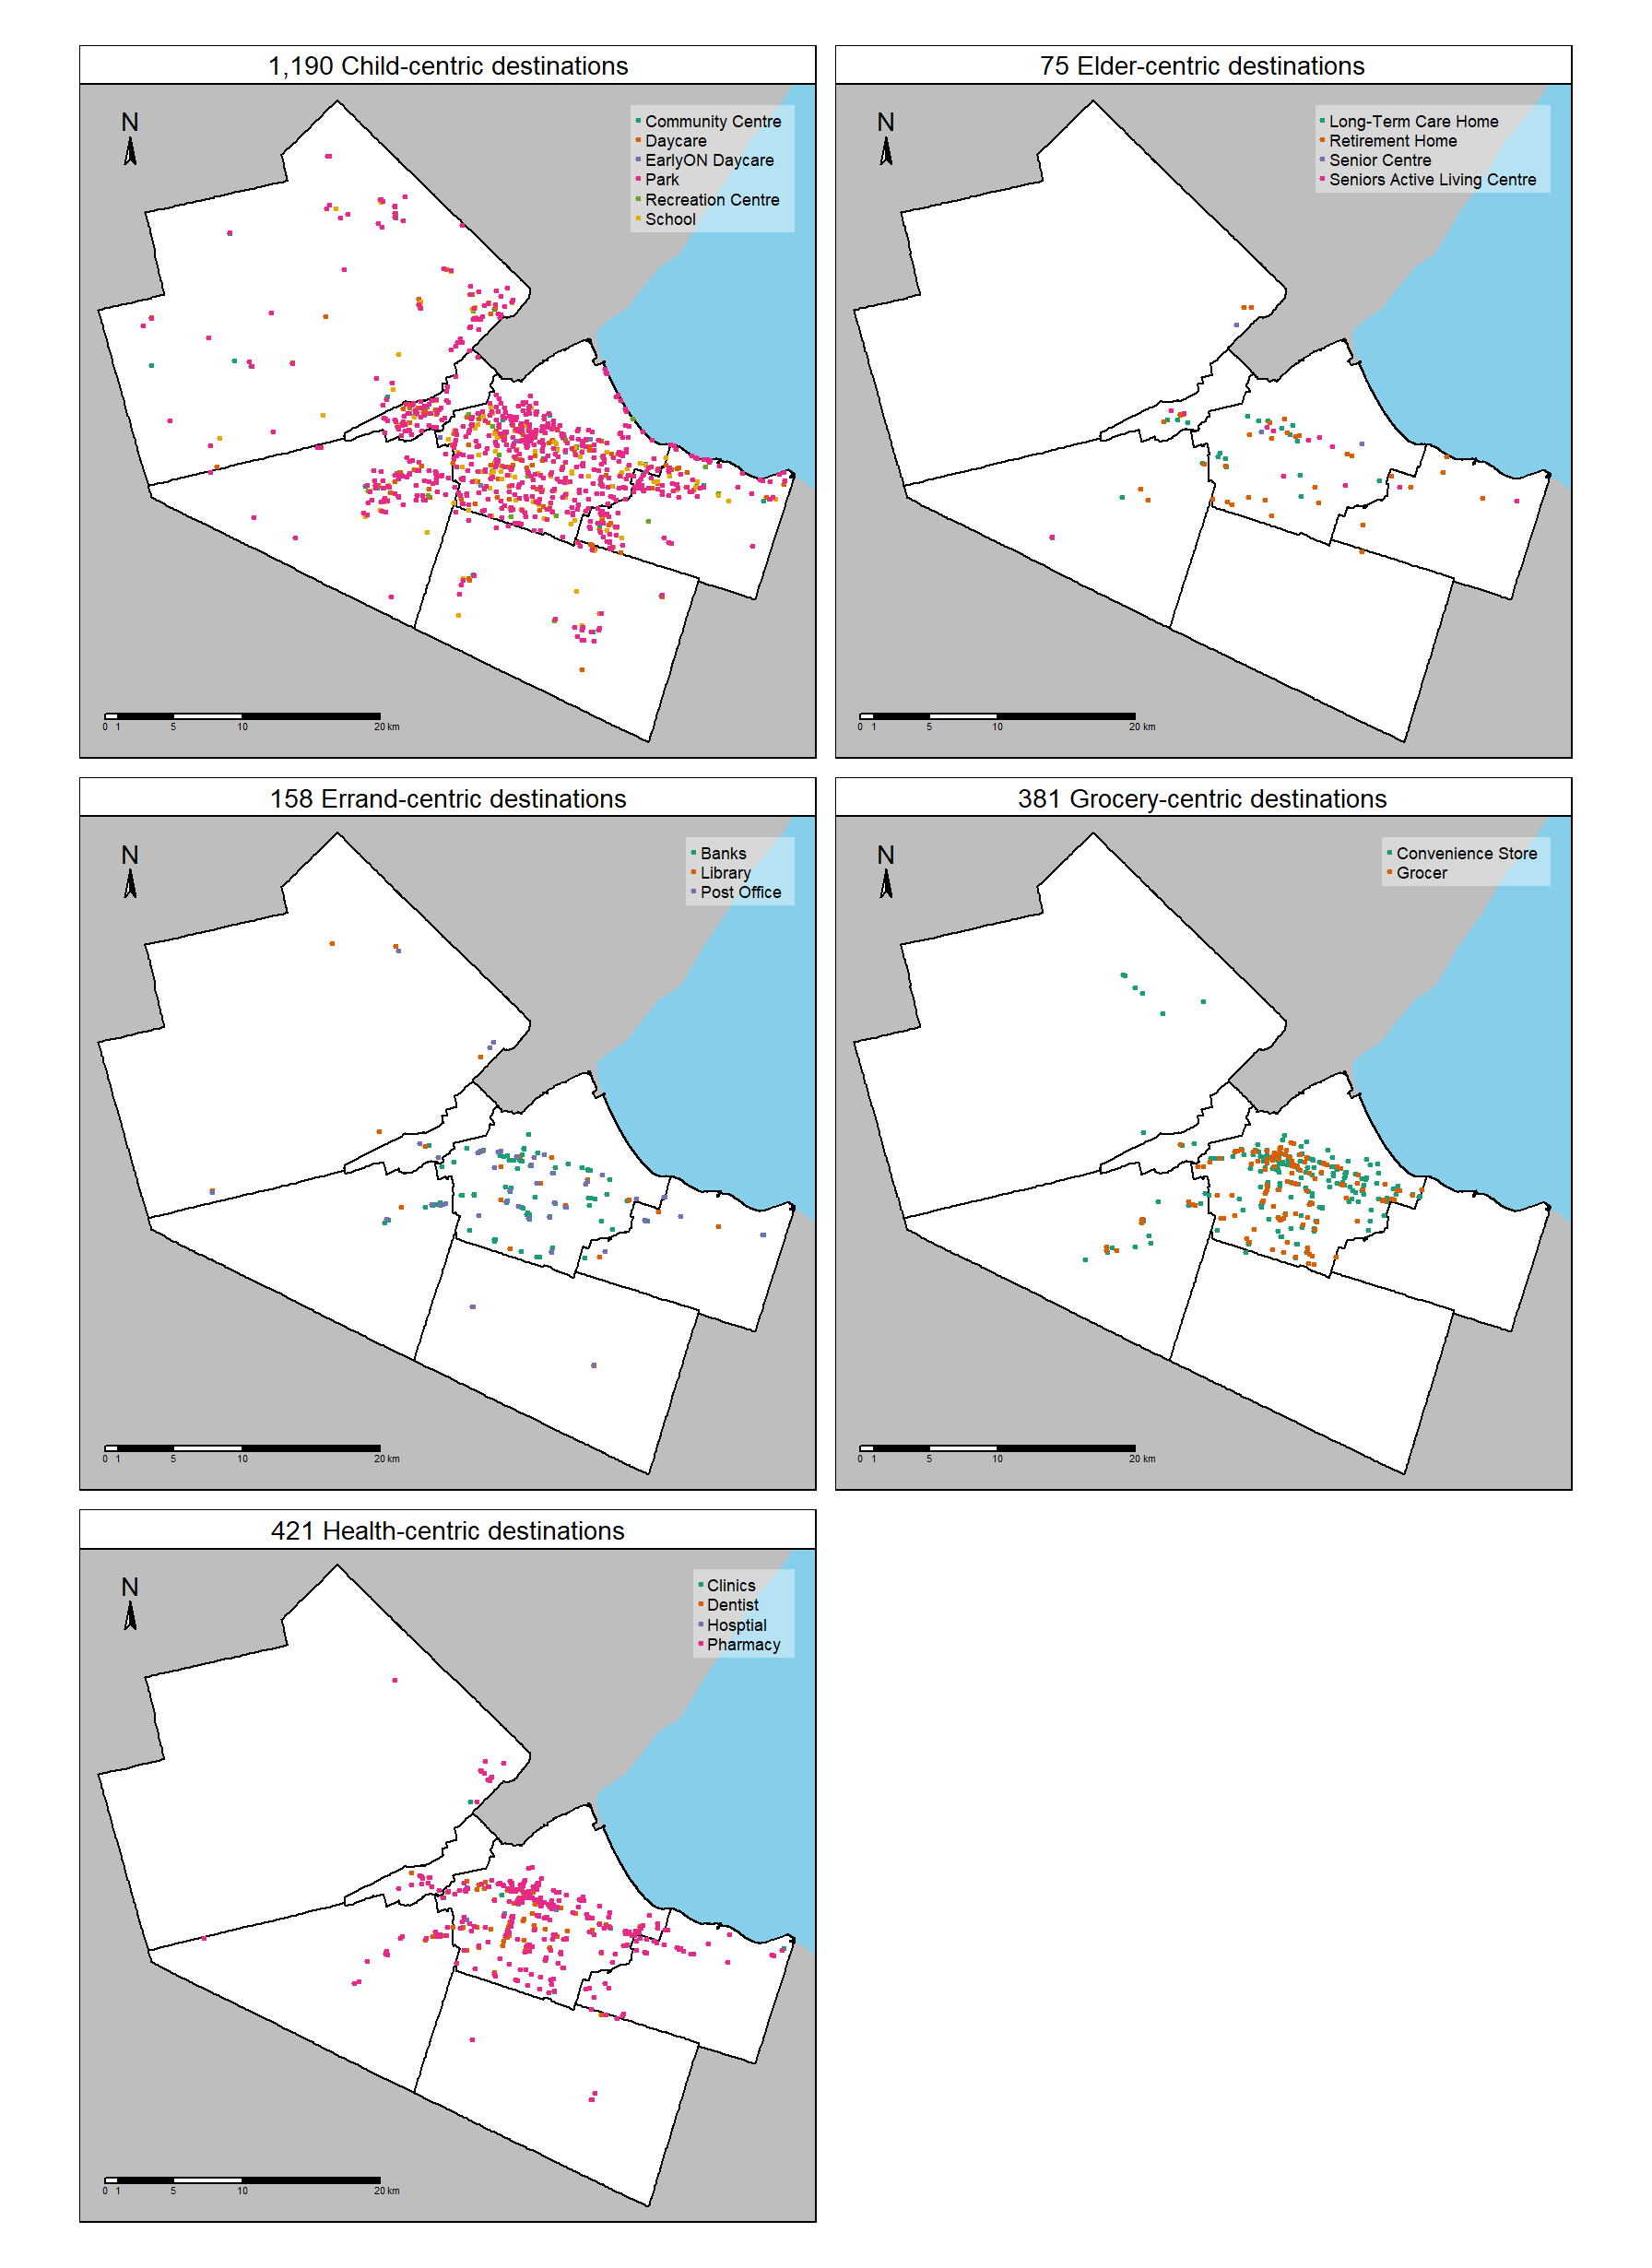
\includegraphics[width=6.25in,height=\textheight]{figures/Fig2-plot_care_categories.png}

}

\caption{\label{fig-Fig2}Locations of care destinations in the City of
Hamilton tagged by the author-generated categories of: child-, elder-,
errand-, grocery- and health- centric care categories. Locations of
these destinations were retrieved through multiple sources as described.
Basemap shapefiles are sourced from the Open Data Hamilton Portal
\citep{opendatahamiltonCityBoundary2023} and the USGS
\citep{greatlakesUSGS2010}.}

\end{figure}%

\subsection{Population data}\label{population-data}

To supplement the care destination dataset and complete the
accessibility calculation (discussed in Methods Section 4), population
data for the City of Hamilton is sourced from the 2021 Canadian census
using the \{cancensus\} R Package
\citep{governmentofcanadaCensusPopulation2023, vonbergmannCancensusCensusMapper2021}.
Three categories of variables are selected: the population, the percent
of after-tax low-income-cut-off (LICO), and the primary commute mode
used. LICO is a composite indicator that reflects the proportion of
households spending 20\% more than the area average on food, shelter and
clothing \citep{governmentofcanadaLowIncomeCutoffs2023}. As stated in
the Introduction Section 1, women, especially those in low-income
households, preform the majority of care trips. However, since the
proportion of women and men residing across the city is balanced, this
study focuses on the total population and total LICO prevalence. All
data was sourced at the most granual level of spatial resolution
publicly available, the level of the dissemination area (DA).

Figure~\ref{fig-Fig3} displays the spatial distribution of the total
population and LICO as a percentage of the total population. Notably,
the density of population within Hamilton-Central (oranges) and the
cluster of high density and high LICO prevalence near the shoreline in
Hamilton-Central (dark purple-oranges).

\begin{figure}

\centering{

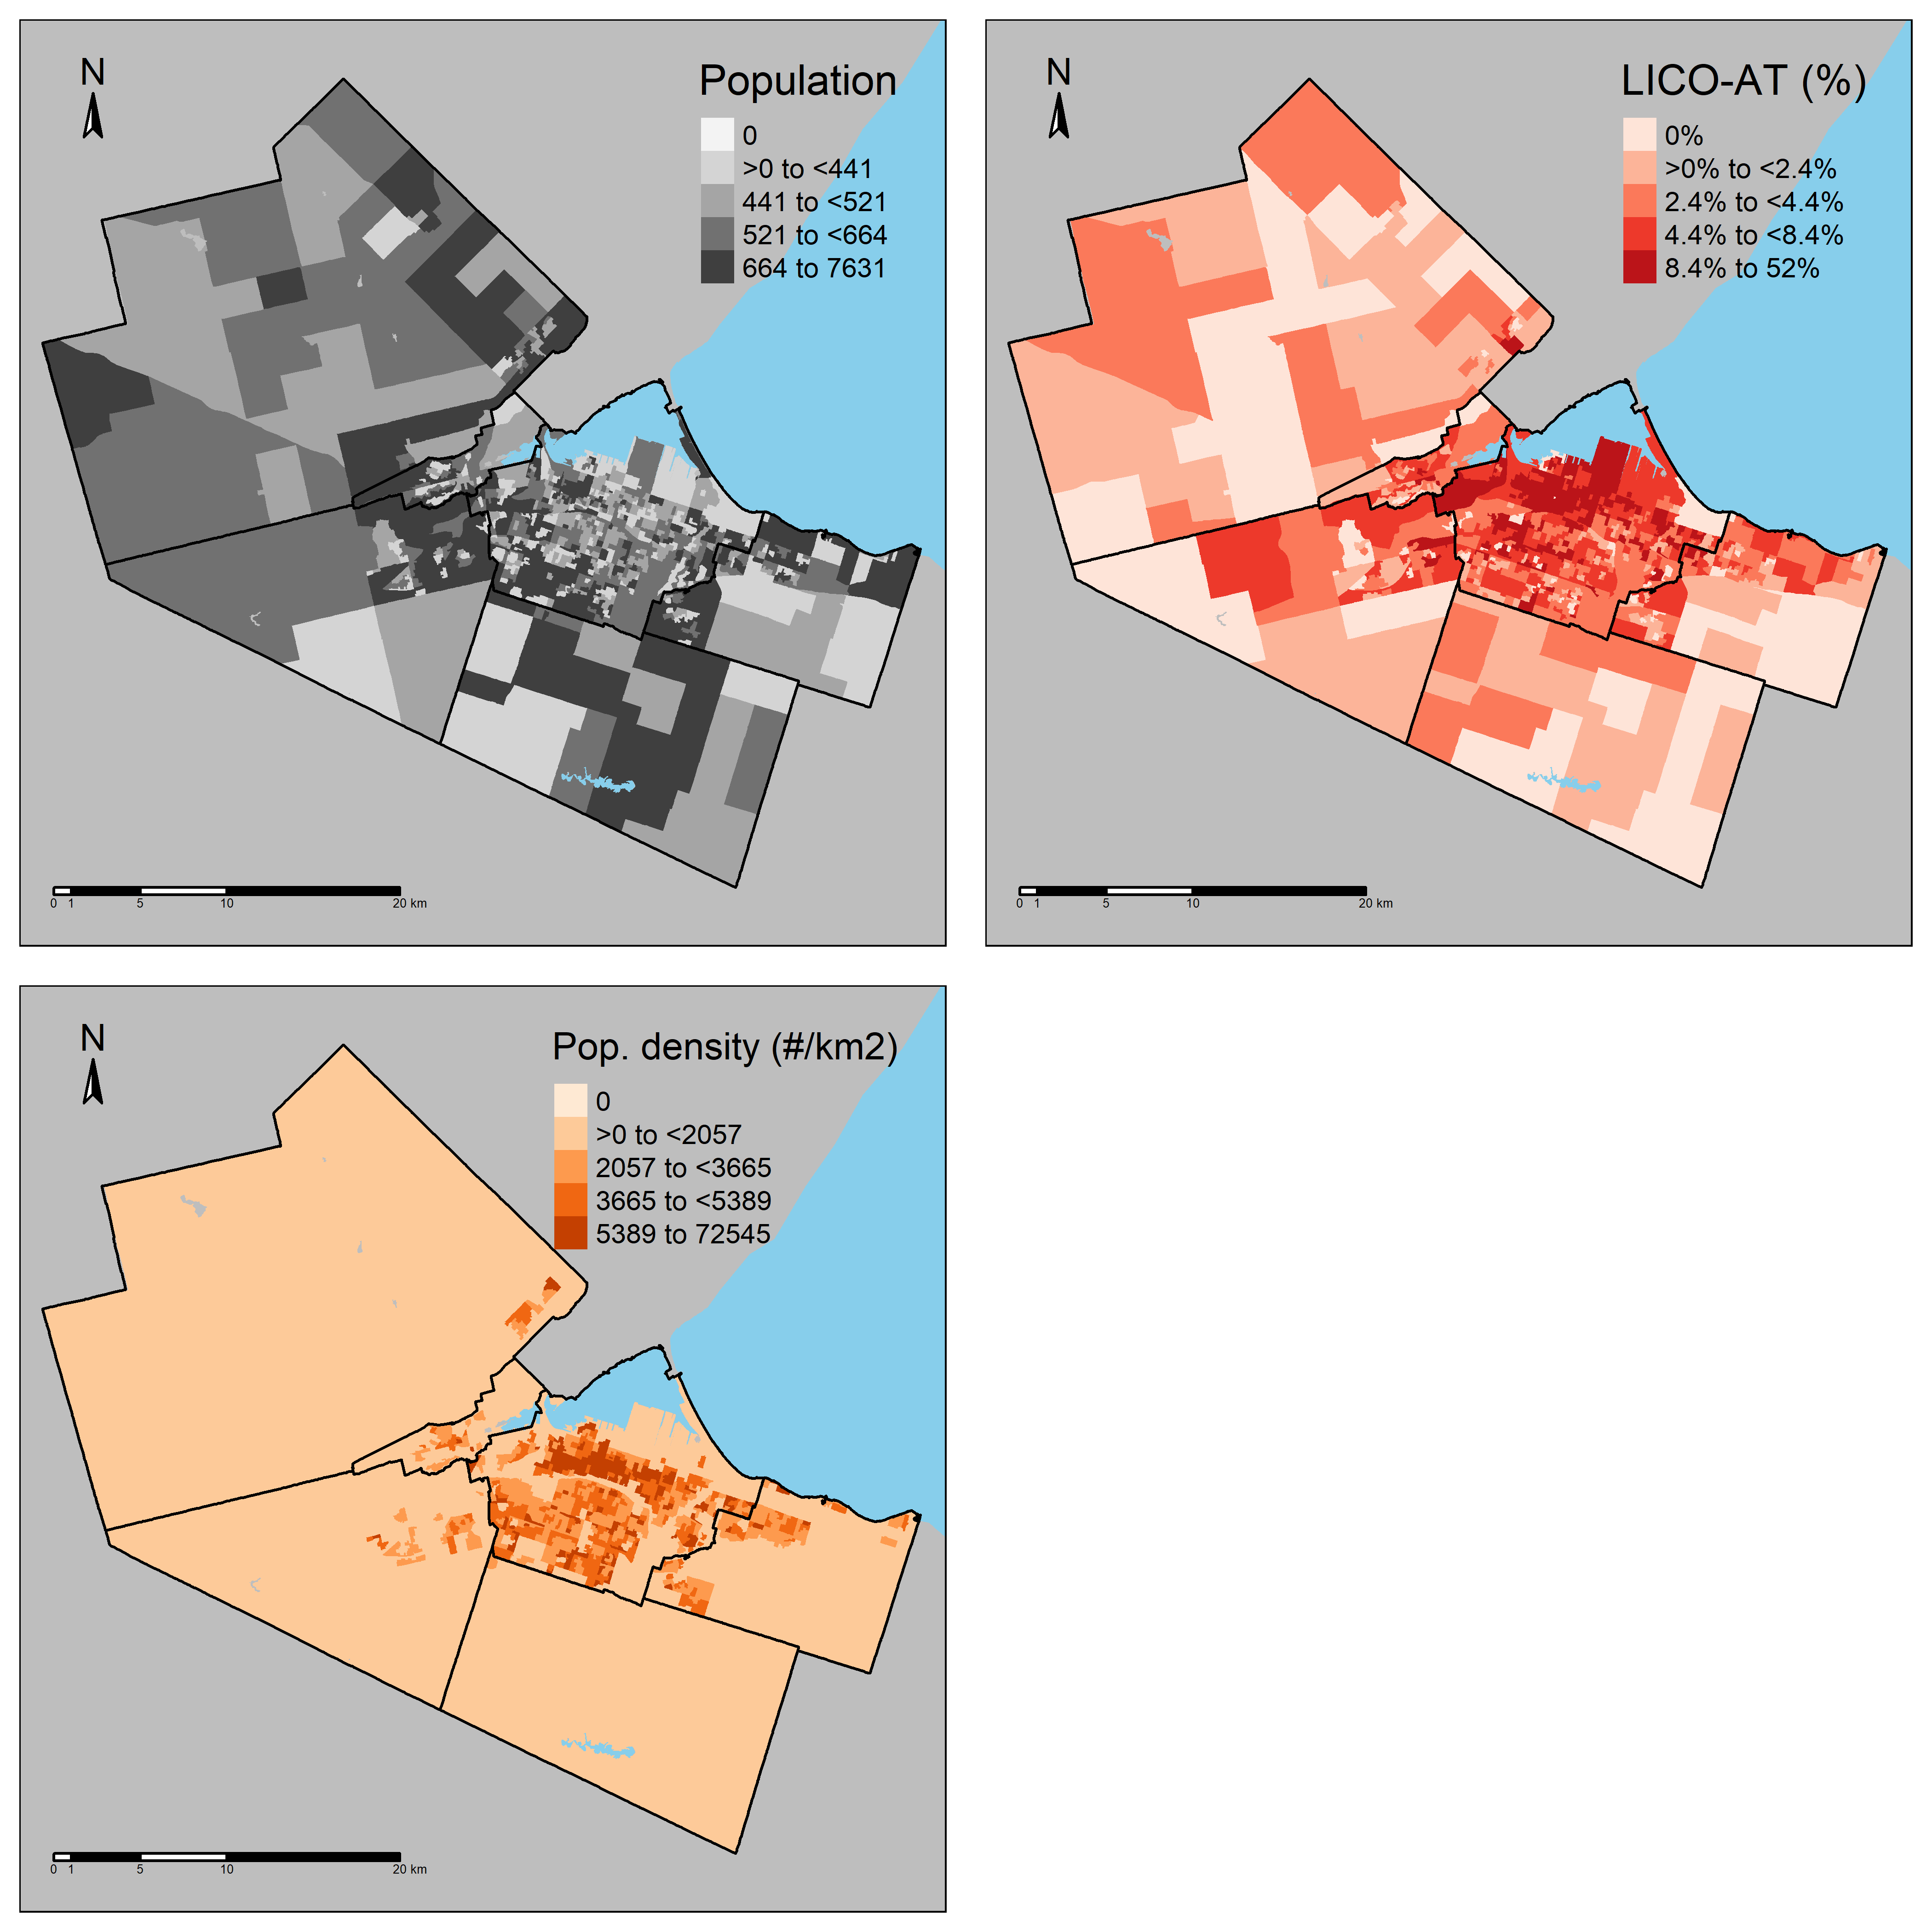
\includegraphics[width=6.25in,height=\textheight]{figures/Fig3-plot_pops.png}

}

\caption{\label{fig-Fig3}The total population in each dissemination area
(DA), visualized with the six former muncipal boundaries in the city of
Hamilton. The left plot represents the population (legend represents
quartiles) and the right represents population density versus the
low-income cut-off after taxes (LICO) as a percentage of the total DA
population. Basemap shapefiles are retrieved from the 2021 Canadian
census \citep{governmentofcanadaCensusPopulation2023}, the Open Data
Hamilton Portal \citep{opendatahamiltonCityBoundary2023} and the USGS
\citep{greatlakesUSGS2010}.}

\end{figure}%

Further, the population proportion that commutes by a specific mode
(car, transit, walk, or cycle/other) is visualised in
Figure~\ref{fig-Fig4}. Though mode choice used in travel to work is not
necessarily reflective of the mode used to travel to care destinations,
no other data is available at a granular level City-wide that captures
mobility of care travel to our knowledge. The population generally
commutes by car (50\% or higher, is yellow to green), even within the
more densely populated Hamilton-Central. However, for transit and
walking, a grouping of DAs near the shoreline within Hamilton-Central
have the highest proportion of transit users and those who walk to work
(yellows in the plots that are otherwise red i.e., below 15\%). Those
same DAs are also relatively dense and have a high prevalence of LICO.

\begin{figure}

\centering{

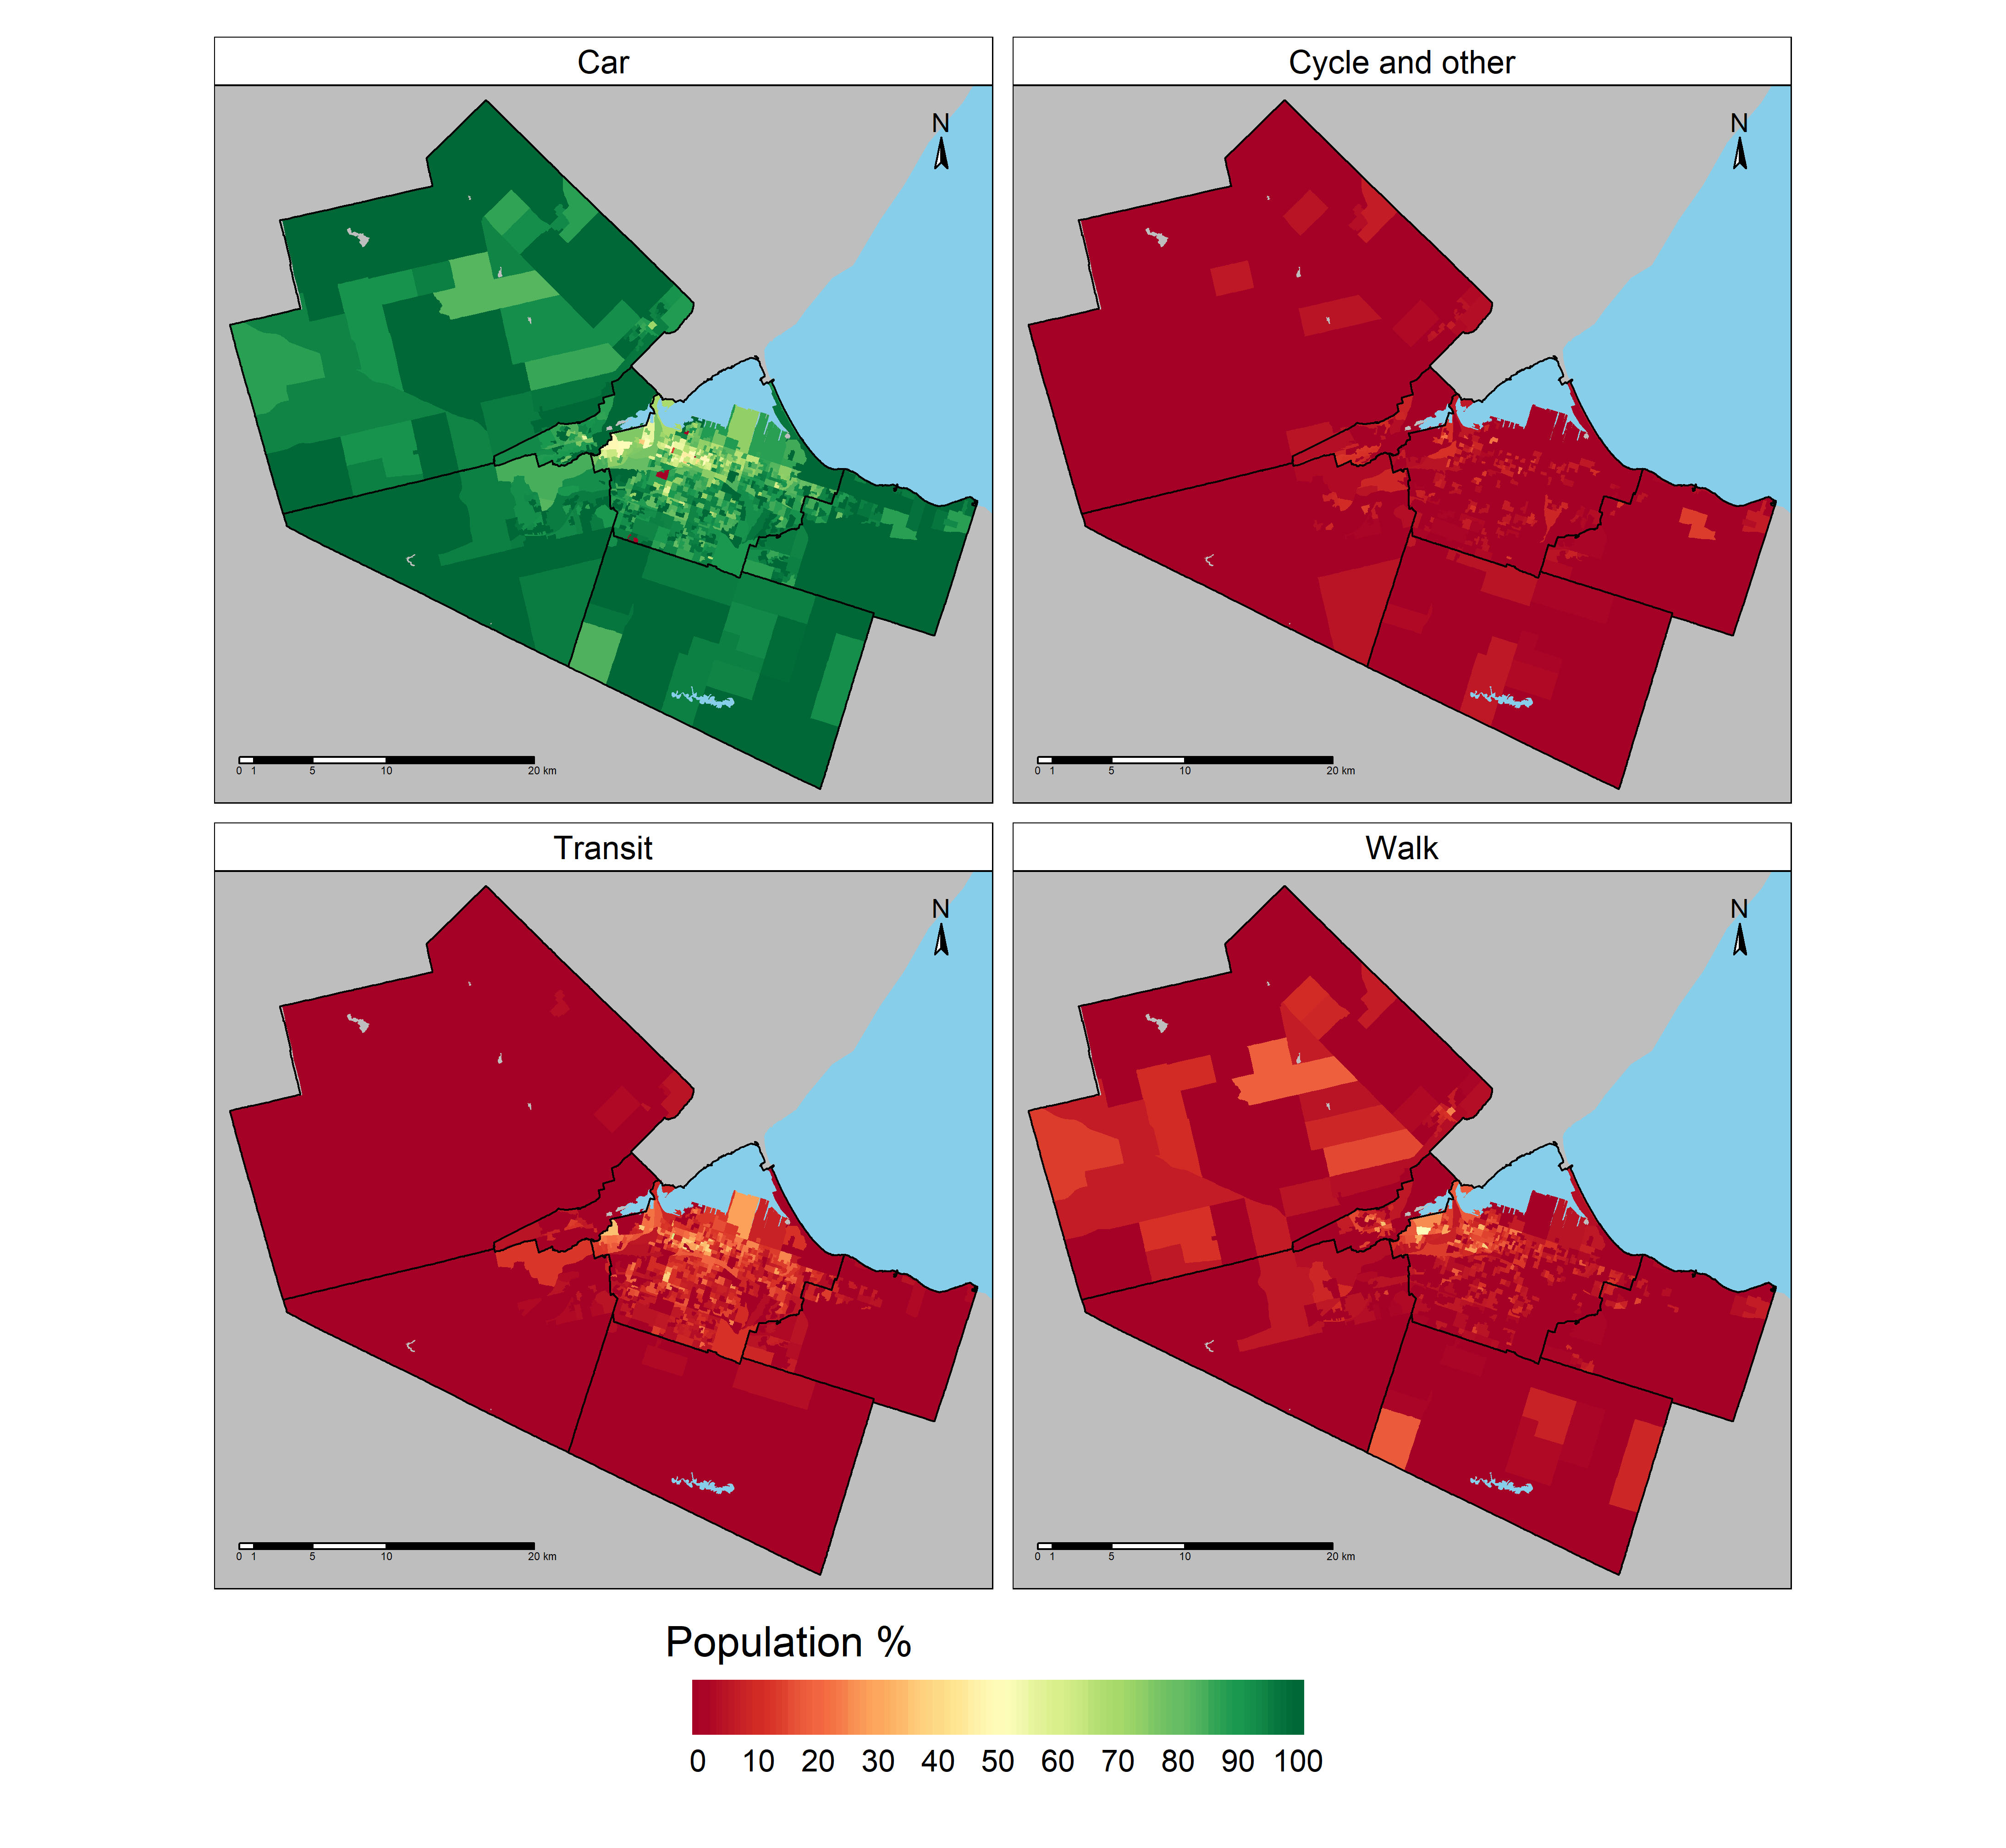
\includegraphics[width=6.25in,height=\textheight]{figures/Fig4-plot_modal_splits.png}

}

\caption{\label{fig-Fig4}The proportion of mode type used for commuting
(aged 15 and older employed in the labour force) in each dissemination
area (DA) as provided by the 2021 Canadian census. Basemap shapefiles
are retrieved from the 2021 Canadian census
\citep{governmentofcanadaCensusPopulation2023}, the Open Data Hamilton
Portal \citep{opendatahamiltonCityBoundary2023} and the USGS
\citep{greatlakesUSGS2010}.}

\end{figure}%

\subsection{Transportation network and travel time
estimations}\label{transportation-network-and-travel-time-estimations}

Travel time to care destinations by walking, cycling, transit and car is
approximated using the `travel\_time\_matrix()' function from the
\{r5r\} package \citep{pereiraR5rRapidRealistic2021}. Inputs into the
function are locations of DA centroids (origins), care destinations
centroids, an OpenStreetMap road network including bike, transit and
vehicle infrastructure \citep{geofabrikOntarioCanadaOpen2023}, and city
GTFS transit routes/schedules
\citep{transitfeedsHamiltonStreetRailway2023}. For all modes, travel
times under 60 minutes based on the shortest travel-time path are
calculated.

For transit and cycling, additional parameters were included. For
transit travel times, a Wednesday departure time of 8:00AM was selected
\citep{boisjolyDailyFluctuationsTransit2016} with a departure travel
window parameter of 30 mins. Travel times are calculated for each minute
of the travel window (8:00-8:30AM) and the 25th percentile from the
distribution of travel window times were selected to represent each
origin-destination. Selecting a sufficiently wide window is an important
consideration as travel times are sensitive to transit vehicle frequency
and connecting transfers (see discussion of the modifiable temporal unit
problem e.g., \citep{pereiraFutureAccessibilityImpacts2019}). The 25th
percentile indicates that 25\% of trips from that origin to destination
have a travel time that is that length or shorter. This assumption
provides a more optimistic perspective on transit travel times. For
cycling travel times, level 1 or 2 level of traffic stress (LTS) routes
(i.e., dedicated or separated cycling lanes, respectively) were
selected. The LTC is a calculated variable associated with links of the
OSM road network. LTS 1 and 2 are considered mainstream cycling
conditions \citep{faghihimaniCycleAccessibilityLevel2019} and are the
function's default.

\section{Accessibility measurement
methods}\label{accessibility-measurement-methods}

Two accessibility measures are detailed: the cumulative opportunity
measure and the spatial availability measure. Both yield a value per
spatial unit that represents how many care destinations can be reached
within a given travel time, for a given mode. However, both measures
have different underlying assumptions; the first does not consider
competition effects and the second does.

\subsection{Cumulative opportunities: the number of care opportunities
that can be reached by a mode within a travel
time}\label{cumulative-opportunities-the-number-of-care-opportunities-that-can-be-reached-by-a-mode-within-a-travel-time}

Often referred to as the cumulative opportunity measure, it is a special
form of the gravity-based accessibility measure
\citep{handyMeasuringAccessibilityExploration1997}. It receives its name
from its interpretation: the value calculated for each spatial unit (DAs
in this study) represents the number of opportunities that could be
spatially accessed within a given travel time. The cumulative
opportunity accessibility measure takes the following general form for a
multimodal calculation: \begin{equation}\phantomsection\label{eq-1}{
S_i^m=\sum_{j}O_j\cdot f^m(c_{ij}^m)
}\end{equation} \noindent Where:

\begin{itemize}
\tightlist
\item
  \(i\) is a set of origin locations (e.g., DA centroids)
\item
  \(j\) is a set of destination locations (e.g., care destinations)
\item
  \(m\) is a set of modes (e.g., by foot, cycle, transit and car)
\item
  \(O_j\) is the number of opportunities at \(j\) (e.g., in this study,
  the presence of a care destination)
\item
  \(c_{ij}^m\) is the travel cost between \(i\) and \(j\) for each
  \(m\).
\item
  \(f^m(\cdot)\) is an impedance function of \(c^m_{ij}\) for each
  \(m\); within the cumulative opportunity measure, it is a binary
  function that takes the value of 1 if \(c^m_{ij}\) is less than a
  selected value.
\item
  \(S^m_{i}\) is the cumulative opportunities accessible by \(m\) at
  each \(i\).
\end{itemize}

\subsection{Spatial availability: the number of care opportunities that
are spatially available to a mode-user within a travel
time}\label{spatial-availability-the-number-of-care-opportunities-that-are-spatially-available-to-a-mode-user-within-a-travel-time}

Differing from cumulative opportunity measure, the spatial availability
measure considers competition. The spatial availability value for each
origin \(i\) for a given mode \(m\) represents the number of care
opportunities that can be accessed by a mode-user out of \emph{all} care
opportunities in Hamilton. Spatial availability considers competition
through the proportional allocation of opportunities to a given \(i\).
The proportional allocation balancing factors are based on the relative
proportion of population computing for an opportunity and their travel
times to reachable destinations.~Spatial availability, takes the
following general form for multi-modal calculation:
\begin{equation}\phantomsection\label{eq-2}{
V^m_{i} = \sum_{j} O_j\ F^{tm}_{ij}
}\end{equation} \noindent Where:

\begin{itemize}
\tightlist
\item
  Like in Equation~\ref{eq-1}, \(i\), \(j\), and \(m\) is a set of
  origin locations, destination locations, modes respectively and
  \(O_j\) is the number of opportunities at \(j\).
\item
  \(V^m_{i}\) is the cumulative opportunities spatially available by
  \(m\)-using population at \(i\) for each \(i\).
\item
  \(F^{tm}_{ij}\) is a total balancing factor for each \(m\) at each
  \(i\); it considers the size of the populations at different locations
  that demand opportunities \(O_j\), as well as the cost of movement in
  the system \(f(c_{ij})\).
\end{itemize}

What makes spatial availability stand apart from other competitive
measures is the multimodal balancing factor \(F^{tm}_{ij}\)
\citep[see][]{soukhovMultimodalSpatialAvailability2024, soukhovIntroducingSpatialAvailability2023}.
\(F^{tm}_{ij}\) implements a proportional allocation mechanism that
ensures the sum of all spatial availability values at each \(i\) always
matches the total number of opportunities in the region. In other words,
it ensure an opportunity-side (single) opportunities remain constrained
such that the sum of \(V^m_{i}\) for all \(m\) at each \(i\) is
equivalent to the total sum of opportunities in the region (i.e.,
\(\sum_j O_j = \sum_i V_i = \sum_{m} \sum_{i} V^m_{i}\)). This
constraint helps in clarifying the interpretation of the \(V^m_{i}\)
value itself.

The total proportional allocation factor \(F^{tm}_{ij}\) consists of two
parts: the first is a population-based proportional allocation factor
\(F_i^{pm}\) that models the mass effect (relative population-demand for
opportunities) and the second is an impedance-based proportional
allocation factor \(F_{ij}^{cm}\) that models the cost effect (relative
travel time). Both factors consider competition through proportional
allocation: \(F^{pm}_{i}\) estimates a proportion of how many people are
in each \(i\) and using each \(m\) relative to the region and
\(F^{cm}_{ij}\) estimates a proportion of the cost of travel from \(i\)
to \(j\) at each \(i\) using each \(m\) relative to the region. Both
factors are combined to create the total balancing factor
\(F^{tm}_{ij}\) used to calculate \(V^m_i\):

\begin{equation}\phantomsection\label{eq-3}{
F^{tm}_{ij} = \frac{F^{pm}_{i} \cdot F^{cm}_{ij}}{\sum_{m} \sum_{i} F^{pm}_{i} \cdot F^{cm}_{ij}}
}\end{equation} \noindent Where:

\begin{itemize}
\tightlist
\item
  The factor for allocation by population for each \(m\) at each \(i\)
  is \(F^{pm}_{i} = \frac{P_{i}^m}{\sum_{m}\sum_{i} P_{i}^m}\). This
  factor makes opportunities available based on demand.
\item
  The factor for allocation by cost of travel for each \(m\) at \(i\) is
  \(F_{ij}^{cm} = \frac{f^m(c_{ij}^m)}{\sum_{m} \sum_{i} f^m(c_{ij}^m)}\).
  This factor makes opportunities available preferentially to those who
  can reach them at a lower cost.
\end{itemize}

\subsection{Travel impedance function}\label{travel-impedance-function}

A uniform binary travel impedance function \(f^m(c_{ij}^m)\) is assumed;
specifically, when \(c_{ij}\) is equal or below a certain travel time
threshold, \(f^m(c_{ij}^m)\) equals 1, otherwise, \(f^m(c_{ij}^m)\)
equals 0. Two travel time thresholds are selected for both measures: 15
minutes and 30 minutes for all modes.

This selection is informed by a scan of the literature. Typically,
literature considers travel to one type of care category (e.g., health,
or school, or grocery stores) and each destination type is associated
with varied travel impedance behaviour. As examples, grocery shopping
trips are on average 15 in \citet{hamrickTimeCostAccess2012}, trips to
receive cancer treatments are on average 23.6 minutes for non-white
metro residents in \citet{segelRuralurbanDifferencesAssociation2020}{]},
travel time thresholds of 10 mins are selected for a daycare analysis in
\citet{fransenCommuterbasedTwostepFloating2015}, and 30 mins to 1 hr
travel time thresholds are selected for hospitals in
\citet{schuurmanDefiningRationalHospital2006}. Travel times also depend
on the mode used. From the perspective of mobility of care, average
travel times to all different categories of care destinations are on
average 16 minutes by car and 36 minutes by public transportation
\citep{ravensbergenExploratoryAnalysisMobility2022}. To broadly reflect
this past research: 15 and 30 minutes are selected in this study.

As previously discussed, the use of binary travel impedance functions as
opposed to distance decay impedance functions was selected to simplify
communication of the assumed travel behaviour. Lacking region-specific
empirical data regarding care-centric travel, this work establishes a
methodology to streamline access to care interpretation and analysis for
when that data is available.

\section{Results}\label{results}

\subsection{Cumulative opportunities: access to
care}\label{cumulative-opportunities-access-to-care}

The cumulative opportunity and spatial availability plots for each mode
and 15-minute and 30-minute travel time thresholds are shown in
Figure~\ref{fig-Fig5}. Each cumulative opportunities value represents a
cumulative count of care opportunities that can be spatially accessed by
each mode from each DA, where each opportunity represents a reachable
care destination. The spatial availability measure presents a
constrained interpretation of this measure; each value is a cumulative
count of care opportunities that can be spatially accessed from each DA
and \emph{are spatially available to the mode-using population based on
the relative size of the mode-using population and modal travel times}.
As proportional allocation is used, each spatial availability value can
also be interpreted as the \emph{spatially available} proportion of the
total care destinations in the city, i.e., the sum of all spatial
availability values in the second row of Figure~\ref{fig-Fig5} equal,
the total number of care destinations in this case study.

In both measures, the higher the value, the more potential interaction
with care opportunities. This greater potential of opportunity of
interaction is conceptualised as a positive outcomes of well functioning
land-use and transport networks
\citep{corderaImpactAccessibilityPublic2019, blumenbergDriveWorkRelationship2017, cuiSpatialAccessPublic2020}.
In Figure~\ref{fig-Fig5}, values are grouped by quantile and spatial
trends between the 15-min and 30-min threshold plots are highly
correlated (0.92 for cumulative opportunities and for 0.89spatial
availability).

\begin{figure}

\centering{

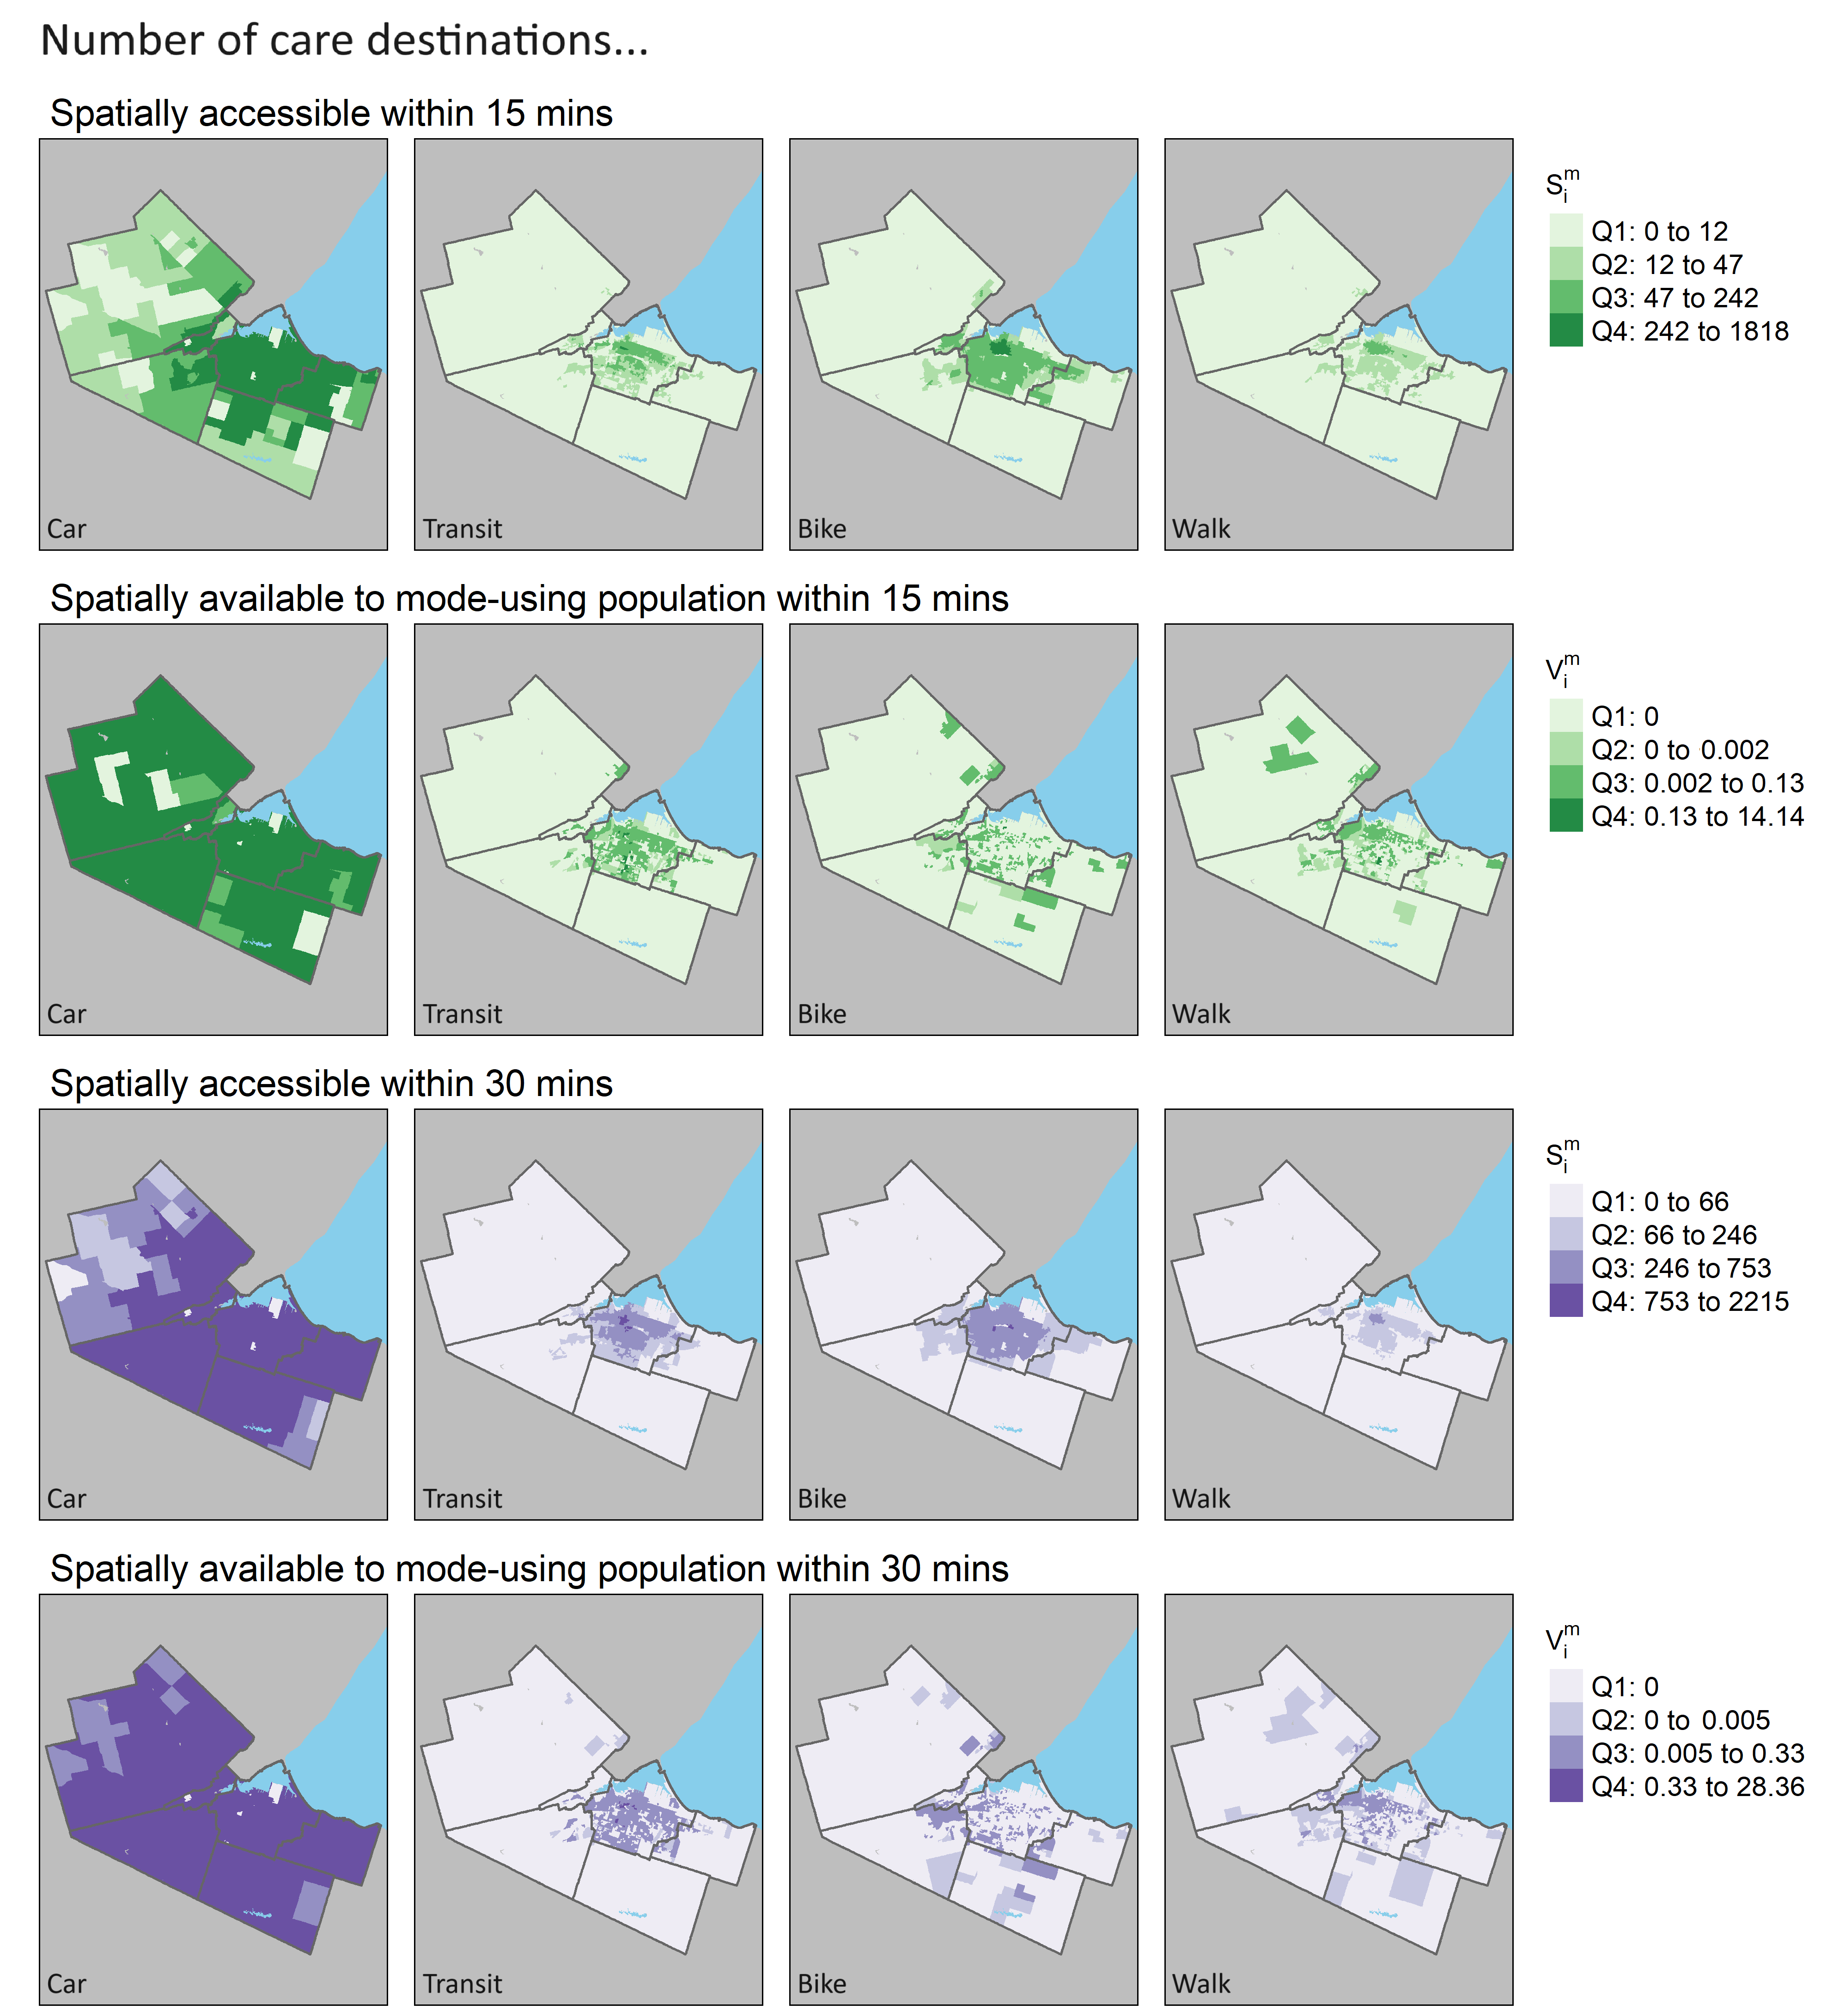
\includegraphics[width=6.25in,height=\textheight]{figures/Fig5-plot_copp_Savail_measures.png}

}

\caption{\label{fig-Fig5}The number of care destinations that can be
reached, per DA, within 15 mins (top) and 30 mins (bottom) for the
cumulative . Basemap shapefiles are retrieved from the 2021 Canadian
census \citep{governmentofcanadaCensusPopulation2023}, the Open Data
Hamilton Portal \citep{opendatahamiltonCityBoundary2023} and the USGS
\citep{greatlakesUSGS2010}.}

\end{figure}%

When considering cumulative opportunity measure; three notable findings
between modes can be identified. First, access by transit and walking is
somewhat high (mostly Q3 and some Q4) within the core of
Hamilton-Central but low elsewhere. This finding is somewhat expected as
as transit does not significantly serve communities outside of
Hamilton-Central and Dundas, and the density of walking infrastructure
is high in Hamilton-Central (see Figure~\ref{fig-Fig1}). Second, access
by cycling is even higher (mostly Q3 but more Q4) in Hamilton-Central;
it provides the second most opportunities for interactions after travel
by car, and affords at least one opportunity for interaction in more DAs
than walking and transit use (notably some access (Q1) in rural
communities). Third, the access that the car-mode provides is
significantly higher relative to the three sustainable modes. Travel by
car results in the greatest maximum number of potential interactions to
care destinations (1818 and 2215 opportunities within 15-min and 30-mins
respectively). Car-mode offering high accessibility to care destinations
is an expected outcome given the car-oriented design of North American
cities \citep{saeidizandRevisitingCarDependency2022} and the range
(travel speeds over a distance) of the car mode. However, though car
ownership is high in Hamilton, not everyone has access to a private
vehicle. For instance, 13\% of Hamilton households do not own a car
\citep{datamanagementgroupTTSTransportationTomorrow2018}, presenting
equity concerns in who may benefit from the high accessibility car-mode
offers. The cumulative opportunities access is insightful in
illustrating the range in which opportunities can be accessed by each
mode based on their travel speed (on available infrastructure); a
summary of each origins' modal opportunity isochrone.

However, the cumulative opportunities measure does not account for
competition effects. Namely, what proportion of the modal opportunity
range is \emph{spatially available} to a mode-user at a given location
when competing for those same opportunities with other mode-users.
Considering competition in this way conjures richer conclusions that
reflects the mode-using population. For instance, consider cycling, a
mode that offers a relatively high range but still smaller than the car.
The cumulative opportunities values in Figure~\ref{fig-Fig5} reflects
this intuition: Q3 and Q4 cumulative opportunities values are present
for cycling in Hamilton-Central, offering the second best cumulative
opportunities after the car. However, bike spatial availability values
depicts a more complex story of opportunity accessibility: it reflect
the mode's opportunity range as well as proportion of mode-using
population and how their range relatively compares to all other modes.
The bike-using population is small (2\% of the population), with many
DAs having no or low proportions of bike-users. Meaning DAs with no
bike-users are proportionally allocated no access to opportunities (zero
spatial availability) and DAs with a small proportion of cyclists have
relatively slow travel speeds compared to the car-using population.
Though bike mode offers a relatively high opportunity range (cumulative
opportunities), because of the low proportion of cyclist and their
opportunity range compared to the \emph{many} other mode-users, they
receive low spatial availability values.

Spatial availability values reflect the proportion of cumulative
opportunities accessibility to the mode user (based on relative
population and travel times), which can be used to shed light on what
mode, and in what region, a mode-using population captures more than its
equal share of spatial availability. Overall, 98\% of the spatial
availability is taken by motorists (destinations within 30-minutes) but
they only represent 87\% of the population. Therefore, they have
disproportionately more availability than their population's presence in
the city. Motorists capture this availability from populations that do
not use cars, and as a result are left with lower spatial availability.
For instance, transit users that have access to destinations within
30-minutes represent 7\% of the population but claim only 2\% of the
spatial availability. Similarly, though cyclists and pedestrians
represent 2\% and 4\% of the population respectively, they only capture
0.3\% (cyclist) and 0.3\% (pedestrian) of the spatial availability. In
other words, if certain mode-users capture a greater proportion of
spatial availability, then there is less spatial availability remaining
for other mode users. Spatial availability does not necessarily have to
align with the cumulative opportunities that the mode offers, it is
simply a constrained version that considers competition by mode-using
populations. As noted, non-car modes have the potential to offer higher
cumulative opportunities (within Hamilton-Central), but as it exists
assuming modal commute shares, the majority of spatial availability to
care destinations can still be captured by motorists even in DAs where
car mode share is under 50\% (such as Hamilton-Central, see proportions
in Figure~\ref{fig-Fig4}.

Taken together, though non-car modes may provide somewhat good access to
care destinations within Hamilton-Central (and some only some access in
rural communities), they do not provide similar levels of available
access (spatial availability). Car-using populations capture more
spatial availability, even in the centre of Hamilton-Central, than all
other modes. Note the lower number of Q3 and Q4 values within and
radiating outwards from Hamilton-Central for non-car modes for
cumulative opportunities measure compared to spatial availability.

\subsection{Spatial availability and low-income
mismatch}\label{spatial-availability-and-low-income-mismatch}

To draw insights on who may reside in DAs where populations are
advantaged with higher modal spatial availability, a cross-tabulation is
visualised in Figure~\ref{fig-Fig6}. The modal spatial availability is
divided by the mode-using population in each DA, resulting in the rate
of modal spatial availability. LICO prevalence is the proportion of
population that falls below the low-income cutoff threshold (see
Figure~\ref{fig-Fig3}). Figure~\ref{fig-Fig6} can be interpreted as
follows: residents who use a specific mode in a ``yellow'' area resides
in a DA that offers below average spatial availability (i.e., below or
equal to the the 50th percentile (median) levels of spatial availability
per mode-using population) and the population within the DA has a high
LICO-prevalence (i.e, 80th percentile or higher (8.4\% or more)).

\begin{figure}

\centering{

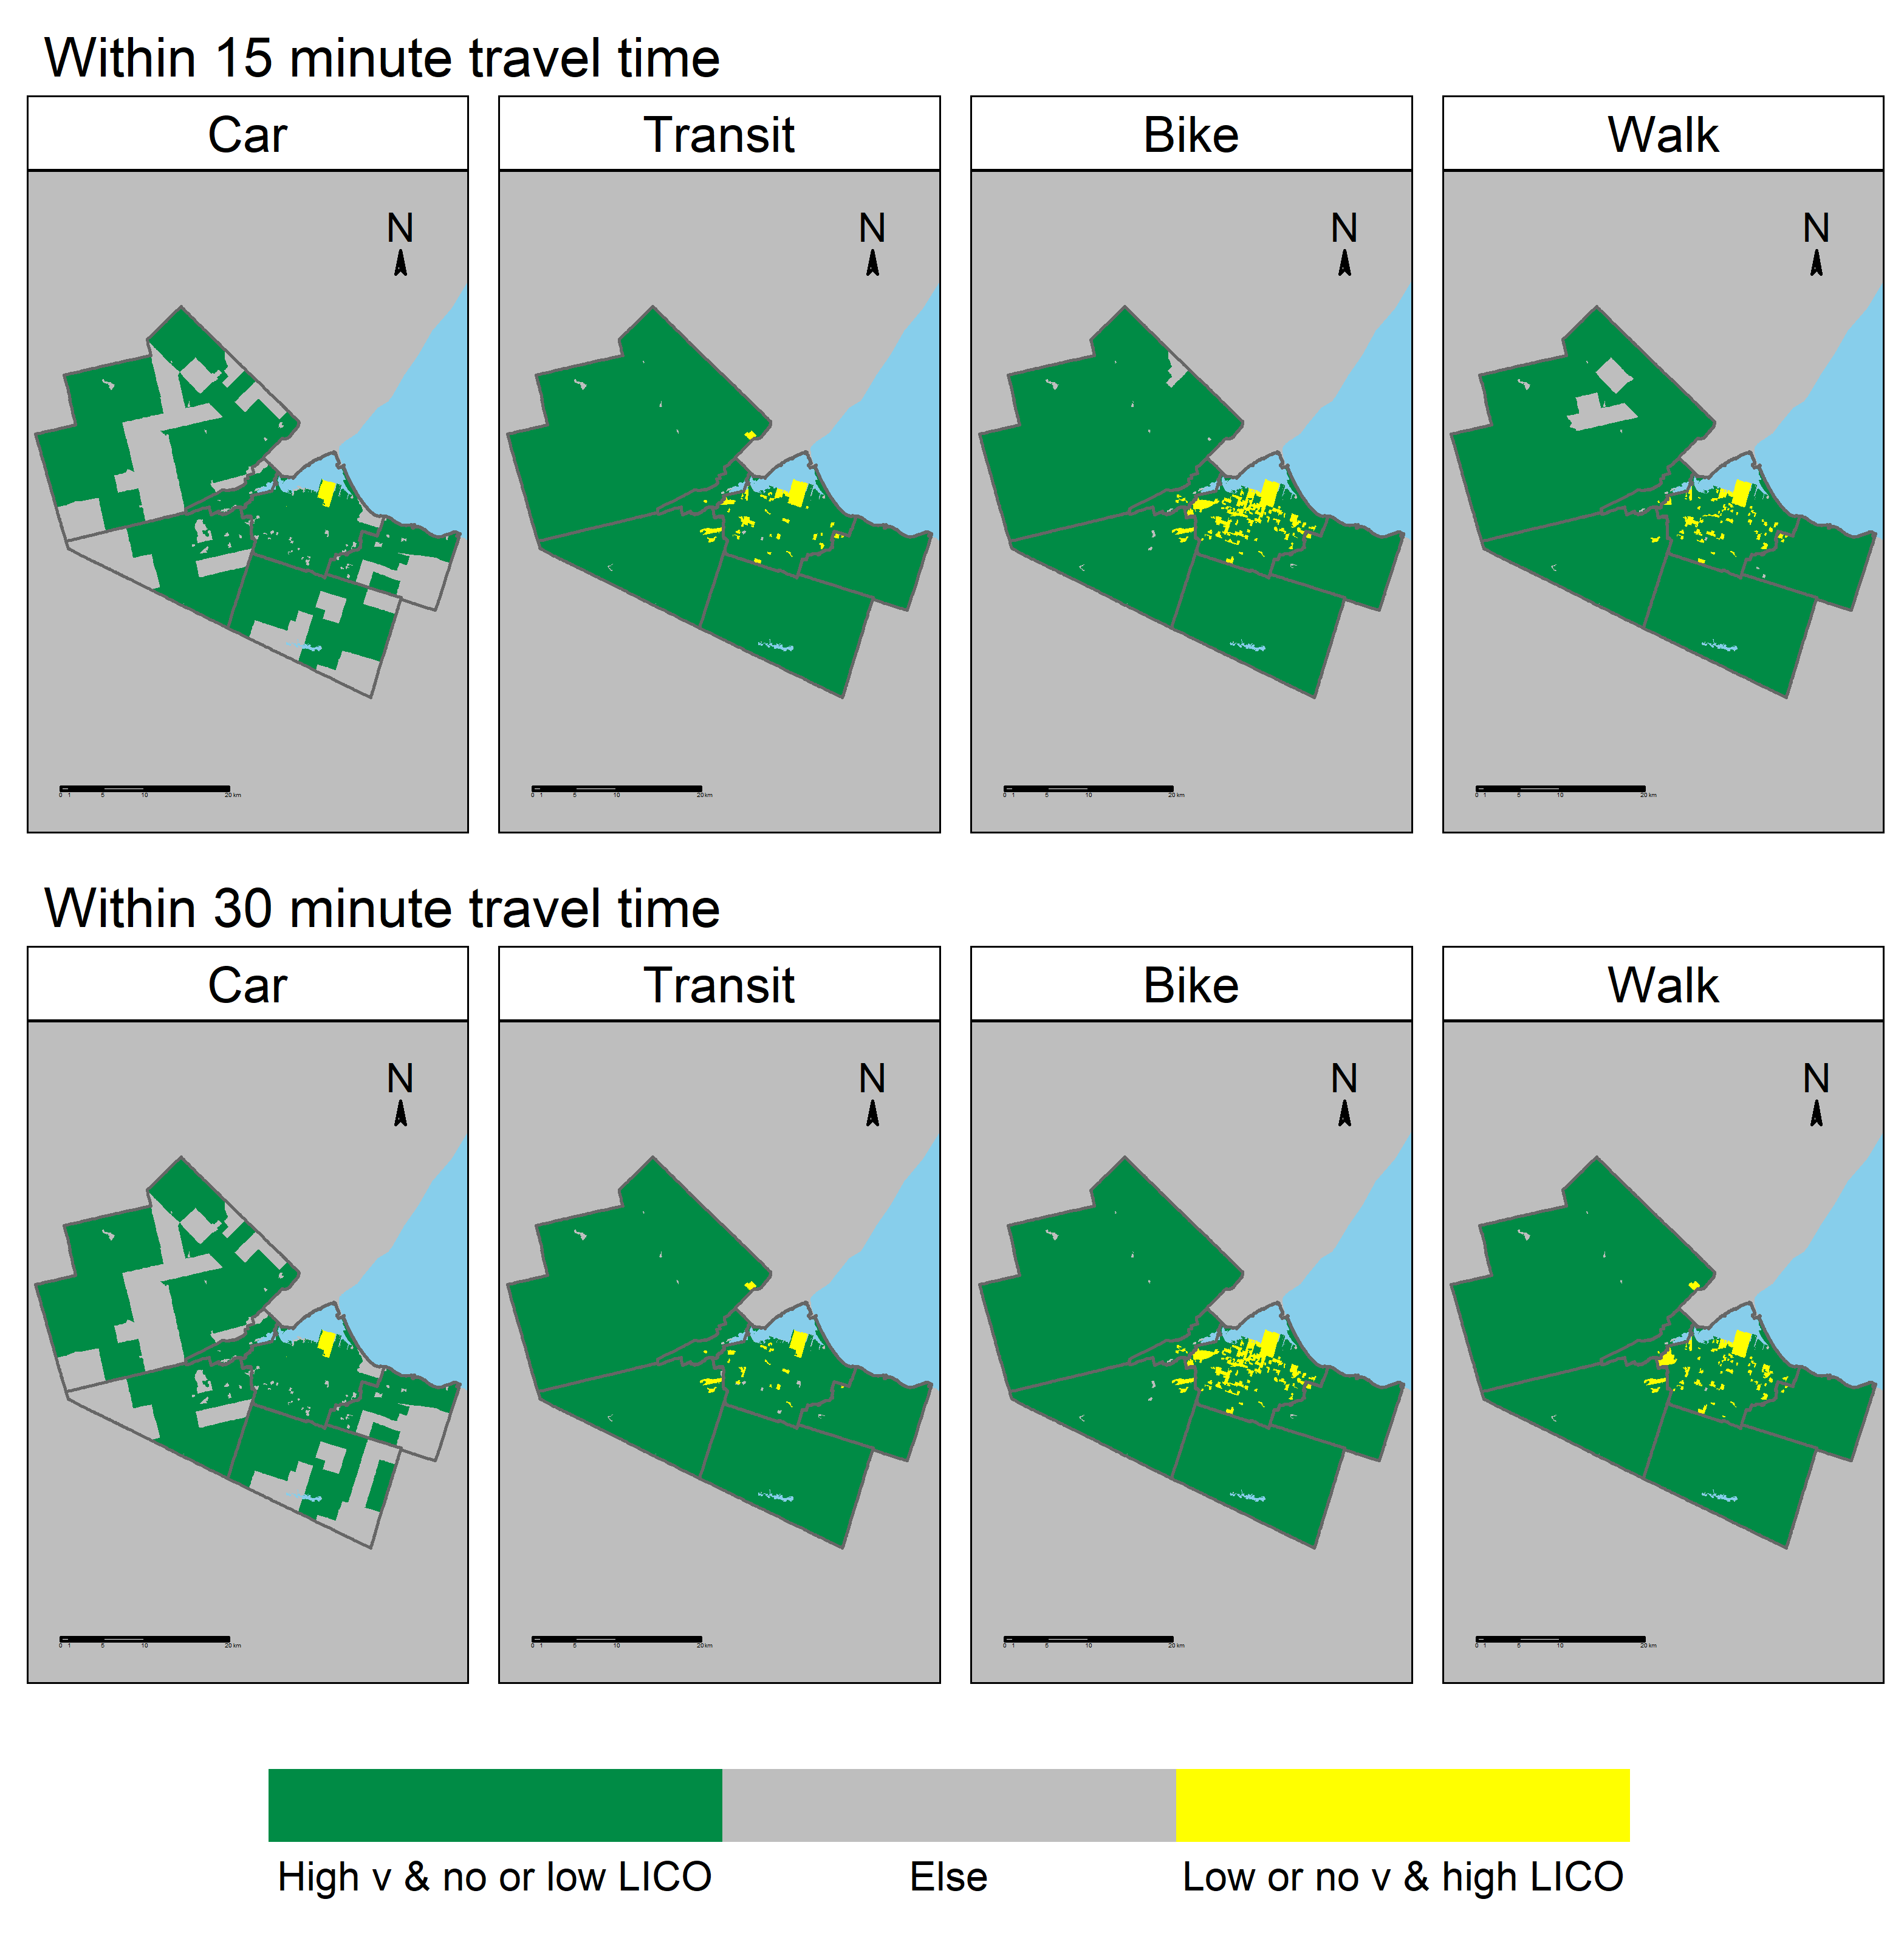
\includegraphics[width=6.25in,height=\textheight]{figures/Fig6-plot_Savail_smallv_LICO_measures.png}

}

\caption{\label{fig-Fig6}The spatial availability per mode-using-capita
measure versus LICO prevelance, visualized for 15 mins (top) and 30 mins
(bottom) travel time cutoffs. Basemap shapefiles are retrieved from the
2021 Canadian census \citep{governmentofcanadaCensusPopulation2023}, the
Open Data Hamilton Portal \citep{opendatahamiltonCityBoundary2023} and
the USGS \citep{greatlakesUSGS2010}.}

\end{figure}%

Notice the green DAs for the car-driving population and presence of
yellow DAs for non-car modes within Hamilton-Central:
Figure~\ref{fig-Fig6} reinforces findings from Figure~\ref{fig-Fig5}.
Even in Hamilton-Central where there is a high proportion of LICO
prevalence, car-mode using populations who reside in green DAs are
offered high levels of spatial availability. However, due to financial
constraints, car ownership is not always possible for low-income
households. Lack of car ownership in areas with insufficient alternative
modes hinders access to economic opportunities
\citep{morrisDoesLackingCar2020, kleinTransitionsOutCar2023}. For this
reason, the introduction of policies that increase availability of care
destination access for non-car modes could be considered. The majority
of yellow DAs are concentrated in the centre of Hamilton-Central for
cycling and walking populations. The mobility of care lens could be used
to further examine policies that improve conditions that decrease LICO
prevalence without displacing local residents, increase the number of
accessible care destinations within Hamilton-Central, and make car-modes
less spatially available (i.e., encourage modal shift, decrease travel
times of non-car modes, and deprioritize decreasing car travel times).

\section{Discussion and conclusions}\label{discussion-and-conclusions}

This paper is the first to conduct an exploratory multimodal
accessibility analysis of Mobility of Care destinations -- one that
counters the current literature's emphasis on employment-related
destinations, a travel purpose more significant for men, and especially
wealthy and educated men
\citep{lawWomenTransportNew1999, hansonGenderMobilityNew2010}. Its aim
is to challenge current planning paradigms by explicitly focusing on
care, vital and life-sustaining activities that are currently
undervalued. This study also provides a tangible example of how one
could conduct a gender-aware multimodal accessibility analyses, using
the city of Hamilton as an empirical case study. In doing so, this paper
contributes to the emergent mobility of care literature, that has
focused on quantifying this underrepresented type of travel
\citep{gomezvaroAccountingCareEveryday2023, murillomunarCaregiversMoveGender2023, ravensbergenExploratoryAnalysisMobility2022, sanchezdemadariagaMobilityCareIntroducing2013, sanchezdemadariagaMeasuringMobilitiesCare2019, shumanCanMobilityCare2023}
through rich and nuanced qualitative accounts of lived experiences
completing mobility of care
\citep{orjuelaReconsideringMobilityCare2023, ravensbergenVelomobilitiesCareLowcycling2020, sersliRidingAloneTogether2020}.

This study also methodologically contributes to the accessibility
literature by contrasting two multimodal accessibility measures: the
widely used cumulative opportunities measure and the spatial
availability measure, which offers accessibility insights on modal
competition. The cumulative opportunities measure demonstrates the modal
range of access by presenting the number of care destinations that each
mode can reach within a 15- and 30- minute travel time threshold from
each spatial location. Spatial availability constrains the cumulative
opportunities measure by incorporating the \emph{assumed} proportions of
mode-using populations and mode-specific travel times; this yields the
number of care destinations that the mode-using population has access to
out of all care destinations in the study region. The two measures
communicate different insights about the case study: the study's results
demonstrate that the car mode offers high cumulative opportunities
access as well as exceptionally high spatial availability for motorists.
While sustainable modes offer lower cumulative opportunities access
(though higher in the city center) and, in certain areas, even lower
spatial availability due to the disproportionately high spatial
availability for the car users. In this way, relying only on the
cumulative opportunities measure could provide an incomplete picture, as
it does not reflect how the relatively large quantity of motorists and
the greater range offered by the car can disproportionately claim more
care destinations than non-car modes (pedestrians, cyclists, and
transit) users. Although spatial availability offers a more complex
picture of how modes provide access under competition, like other
competitive measures, it relies on assumptions about who is
``demanding'' destinations. How those assumptions are made is a subject
of ongoing discussion in the competitive accessibility literature
\citep{merlinDoesCompetitionMatter2017, kelobonyeMeasuringAccessibilitySpatial2020}.

Further, this study contributes to the literature on equitable and
sustainable transportation planning by providing a methodology to
identify areas in need for further development. By highlighting how the
car offers all-round high access and even higher spatial availability to
care destinations in Hamilton, sustainable modes can be prioritized
equitably. Previous research suggests that currently care trips are more
frequently completed by car than by transit or bicycle as they often
involve carrying things (e.g., groceries) or people (e.g., children)
\citep{ravensbergenExploratoryAnalysisMobility2022}. Qualitative work
supports this preference, citing convenience and increased safety as key
reasons for choosing travel by car for care trips
\citep{maciejewskaHaveChildrenThus2019, carverParentalChauffeursWhat2013}.

However, this study also highlights that the high spatial availability
of motorists results in disproportionately low spatial availability for
sustainable mode users, even in Hamilton-Central. While sustainability
policies should aim to re-balance the spatial availability away from
motorists to users of sustainable modes, these policies should
incorporate an equity perspective that considers existing preferences in
care trips. This study provides the stepping stones for such an equity
lens in Figure~\ref{fig-Fig6}, by presenting a cross-tabulation of areas
with high LICO prevalence and low spatial availability per
sustainable-mode that could be the focus of policy intervention.
Consider the cycling plot in Figure~\ref{fig-Fig6}, a factor driving the
higher quantity of yellow DAs is the low proportion of cyclists assumed.
This assumption holds in other Canadian contexts, cycling as a mode for
care trips is also uncommon as cycling is uncommon
\citep{ravensbergenExploratoryAnalysisMobility2022}. Moreover, as care
trips tend to be preformed by women, the low proportion of cycling for
care trips has been put forth as a hypothesis to explain the gender-gap
in cycling observed in low-cycling cities (like Hamilton) where only a
third of cyclists are women
\citep{ravensbergenFeministGeographiesCycling2019, prati2018gender}.
However, cycling as a mode has potential as it demonstrates high
cumulative opportunities values. However, that potential is not being
realized in part due to the low proportion of cyclists and the higher
spatial availability values of motorists. Future research could examine
what barriers those who conduct care trips are facing in regards to
cycling, particularly focusing on the yellow areas indicated in
Figure~\ref{fig-Fig6}.

\subsection{Study limitations}\label{study-limitations}

This study presents three types of limitations related to assumptions in
the accessibility measure methods and data availability. First, since
travel times from origin to care destination are unknown, they are
estimated assuming a road network under free-flow conditions. While this
affects the estimated travel times, research suggests that considering
congested conditions may not significantly impact the resulting
accessibility values \citep{yiannakouliasEstimatingEffectTurn2013}. In
the context of Hamilton, road congestion is also more pertinent to car
and transit modes than for pedestrians or cyclists. Second, using a
binary uniform impedance function instead of a more complex
distance-decay function could significantly affect accessibility results
\citep{kapatsilaResolvingAccessibilityDilemma2023}. For instance,
destinations beyond a 30-minute travel time could still be valued by
people, and those within 5 and 15 minutes do not necessarily have the
same importance. However, the use of the binary function trades
complexity for interpretation, and this trade-off was made strategically
to improve interpretability in the comparison between the two
accessibility measures. To enhance reliability, two literature informed
travel cost thresholds (15-minutes and 30-minutes) are selected. Third,
the geometric centroids of DAs (origins) and destinations (all care
destinations) were used as inputs for travel time calculations. This is
a limitation as DAs were created for the purpose of the statistical
census: they vary in area, and their centroids may not necessarily align
with where that population may begin their journey to care destinations.
This methodological decision presents limitations on how the travel time
estimates can be interpreted to reflect actual travel times to care
destinations.

Moreover, due to the exploratory nature of this research and novelty of
the Mobility of Care concept, no research to date has directly captured
the characteristics of mobility of care trips in Hamilton. The presented
results thus are not calibrated to reflect observed mobility of care
travel behaviour nor establish normative accessibility goals
\citep{paezMeasuringAccessibilityPositive2012}. Travel behaviour data is
needed to calibrate local destination-specific travel impedance cutoffs.
For example, using a 15-minute cutoff for grocery-centric destinations
and a 30-minute cutoff for health-centric destinations or assigning
weights for each destination type as done in previous studies (e.g., a
weight that reflects their ``capacity''
\citep{liMeasuringMultiactivities2024} or their ``attractiveness'' using
origin-destination flows from travel surveys
\citep[\citet{chengInvestigatingWalkingAccessibility2019}]{graellsCityCitiesMeasuring2021}).
In the absence of travel behaviour data and the use of uniform travel
time thresholds and destination weights, the result's interpretation is
limited to the access to \emph{all} care destinations within 15- or
30-minutes. It does not include the real individual socio-economic and
intersectional characteristics that influence what destinations can be
potentially accessed. Consequently, each destination is treated as a
single opportunity, e.g., a school, a clinic, a hospital, and a grocery
store are all equal to one opportunity each. Additionally, since care
trip modal choice is unavailable at a disaggregated level for Hamilton,
the commute mode choice is assumed for the spatial availability measure.
This mode may not be what is used to visit care destinations and hence
places a limitation on how the results should be interpreted.

Taken together, the discussion of these limitations presents room for
future research to incorporate context-specific mobility of care travel
surveys into accessibility analysis to more accurately reflect care
accessibility landscapes. Future work could also look to disaggregate
access to care by category and compare results to access to employment
landscapes. This comparison could highlight the bias in planning toward
jobs, as well as substantiate equity critiques.

\section{Data availability}\label{data-availability}

All work is open, reproducible and completed in R \citep{Rcore}. A
\href{https://github.com/soukhova/Care-Destinations}{GitHub repository}
hosts all associated data, text, figures and code, which relies on the
following R packages: \{knitr\} \citep{knitr1}, \{biscale\}
\citep{biscale}, \{cancensus\} \citep{cancensus}, \{cowplot\}
\citep{cowplot}, \{disk.frame\} \citep{diskframe}, \{dplyr\}
\citep{dplyr}, \{flextable\} \citep{flextable}, \{ftExtra\}
\citep{ftExtra}, \{ggplot2\} \citep{ggplot2}, \{here\} \citep{here},
\{mapview\} \citep{mapview}, \{scales\} \citep{scales}, \{sf\}
\citep{sf2}, \{tmap\} \citep{tmap}, \{tmaptools\} \citep{tmaptools},
\{renv\} \citep{renv}, \{r5r\} \citep{r5r}, \{rlang\} \citep{rlang}, and
\{rmarkdown\} \citep{rmarkdown1}.


\renewcommand\refname{References}
  \bibliography{bibliography.bib}


\end{document}
